%==============================================================================
%  main_rt.tex — Replication-Target draft
%  Layout/structure replicated 1:1 from:
%    Lee KH, Jang S, Kim GJ, et al. "Large Language Models for Automating
%    Clinical Trial Criteria Conversion to Observational Medical Outcomes
%    Partnership Common Data Model Queries: Validation and Evaluation Study."
%    JMIR Med Inform 2025;13:e71252. doi:10.2196/71252
%
%  WHAT IS REPLICATED : section/subsection spine, front matter, structured
%    abstract, 4 figures (incl. A/B dual panels), 5 tables (incl. footnote
%    lettering), statistics repertoire (McNemar / ANOVA / Tukey HSD / chi2 /
%    Cohen d / multiple regression), end matter, running heads, abbreviations.
%  WHAT IS OURS      : every word of content, all data, all figures' data.
%
%  INTEGRITY: numeric results are AUTHOR-SUPPLIED PROVISIONAL values that are
%  internally consistent (every derived quantity recomputes from the tables).
%  They MUST be replaced with the measured run from the compute cluster.
%  Search for "PROVISIONAL" to find every place a measured value goes.
%==============================================================================
\documentclass[10pt]{article}

\usepackage[utf8]{inputenc}
\usepackage[T1]{fontenc}
\usepackage[margin=1in,top=1.05in,bottom=1.05in]{geometry}
\usepackage{times}
\usepackage{amsmath}
\usepackage{amssymb}
\usepackage{graphicx}
\usepackage{booktabs}
\usepackage{array}
\usepackage{xcolor}
\usepackage{caption}
\usepackage{fancyhdr}
\usepackage{enumitem}
\usepackage{tikz}
\usetikzlibrary{shapes.geometric,arrows.meta,positioning,fit,backgrounds,calc}
\usepackage{pgfplots}
\pgfplotsset{compat=1.16}
\usepgfplotslibrary{groupplots}
\usepgfplotslibrary{colormaps}
\usepackage[colorlinks=true,allcolors=blue!55!black]{hyperref}

%---------------- JMIR-like page furniture ----------------
\pagestyle{fancy}
\fancyhf{}
\renewcommand{\headrulewidth}{0.4pt}
\renewcommand{\footrulewidth}{0pt}
\fancyhead[L]{\footnotesize JMIR MEDICAL INFORMATICS}
\fancyhead[R]{\footnotesize \RUNAUTH}
\fancyfoot[L]{\scriptsize \JOURNALURL}
\fancyfoot[R]{\scriptsize\shortstack[r]{%
  \JOURNALCITE\ | p.~\thepage\\[-2pt]\textit{(page number not for citation purposes)}}}
\newcommand{\RUNAUTH}{[First Author] et al}
\newcommand{\JOURNALURL}{https://medinform.jmir.org/XXXX/X/eXXXXX}
\newcommand{\JOURNALCITE}{JMIR Med Inform XXXX | vol.~XX | eXXXXX}
\setlength{\headheight}{13pt}
\setlength{\footskip}{28pt}

%---------------- JMIR-like sectioning (no titlesec dependency) ----------------
\makeatletter
\renewcommand\section{\@startsection{section}{1}{\z@}%
  {2.6ex \@plus 1ex \@minus .2ex}{1.3ex \@plus .2ex}%
  {\normalfont\large\bfseries}}
\renewcommand\subsection{\@startsection{subsection}{2}{\z@}%
  {2.0ex \@plus 1ex \@minus .2ex}{0.9ex \@plus .2ex}%
  {\normalfont\normalsize\bfseries}}
\renewcommand\subsubsection{\@startsection{subsubsection}{3}{\z@}%
  {1.6ex \@plus 1ex \@minus .2ex}{0.7ex \@plus .2ex}%
  {\normalfont\normalsize\itshape}}
\makeatother
\setcounter{secnumdepth}{0}   % JMIR headings are unnumbered

%---------------- captions above floats, "Figure 1." style ----------------
\captionsetup{labelsep=period,font=small,justification=justified,
              singlelinecheck=false,skip=4pt}

%---------------- helpers ----------------
\newcommand{\PH}[1]{{\color{red}\textbf{[#1]}}}
\newcommand{\tnote}[1]{\textsuperscript{#1}}
\newcommand{\tabfoot}[1]{\par\vspace{2pt}\noindent{\footnotesize #1}}
\newcolumntype{L}[1]{>{\raggedright\arraybackslash}p{#1}}
\newcolumntype{C}[1]{>{\centering\arraybackslash}p{#1}}

\begin{document}
\thispagestyle{fancy}

%==============================================================================
%  FRONT MATTER  (replicates JMIR title-page block)
%==============================================================================
\noindent{\large\bfseries Original Paper}

\vspace{6pt}
\noindent{\LARGE\bfseries Large Language Models for Automating Hospital\\[2pt]
Statistical Criteria Conversion to Clinical Data Warehouse\\[2pt]
Queries: Validation and Evaluation Study\par}

\vspace{10pt}
\noindent
\PH{Author One}\textsuperscript{1}, MD, PhD;
\PH{Author Two}\textsuperscript{2}, MSc;
\PH{Author Three}\textsuperscript{2}, BEng;
\PH{Author Four}\textsuperscript{3}, MSc;
\PH{Author Five}\textsuperscript{4}, MD;
\PH{Author Six}\textsuperscript{3}, PhD;
\PH{Author Seven}\textsuperscript{5}, MD, PhD;
\PH{Author Eight}\textsuperscript{1,5}, MD, PhD

\vspace{4pt}
{\footnotesize
\noindent\textsuperscript{1}Department of Medical Informatics, \PH{Hospital Name}, \PH{University}, \PH{City}, China\\
\noindent\textsuperscript{2}Big Data Platform Center, \PH{Hospital Name}, \PH{City}, China\\
\noindent\textsuperscript{3}Department of Anesthesiology and Surgical Management, \PH{Hospital Name}, \PH{City}, China\\
\noindent\textsuperscript{4}Department of Laboratory Medicine and Blood Transfusion, \PH{Hospital Name}, \PH{City}, China\\
\noindent\textsuperscript{5}Department of Quality Management, \PH{Hospital Name}, \PH{University}, \PH{City}, China\par}

\vspace{8pt}
\noindent\textbf{Corresponding Author:}\\
{\footnotesize
\PH{Corresponding Author}, MD, PhD\\
Department of Medical Informatics\\
\PH{Hospital Name}\\
\PH{Street Address}\\
\PH{City} \PH{Postcode}\\
China\\
Phone: \PH{+86 ...}\\
Fax: \PH{+86 ...}\\
Email: \PH{corresponding@example.edu}\par}

%------------------------------ ABSTRACT ------------------------------
\section*{Abstract}
\noindent\textbf{Background:} Hospital information systems accumulate years of
operational data whose table joins and, above all, whose statistical
\emph{criteria}---which timestamp a case is counted by, which flag defines an
indicator---are strongly institution-specific. Analysts express reporting needs in
free text, but retrieval still depends on engineers hand-writing SQL, and
automating that conversion is hindered by the same two obstacles as any
high-stakes query-generation task: ensuring accuracy and producing outputs an
engineer can audit.

\noindent\textbf{Objective:} The aim of this study is to develop an automated
system converting free-text hospital statistical requests into Presto SQL
queries compatible with a three-layer clinical data warehouse (CDW) and to
systematically evaluate hallucination patterns across multiple large language
models (LLMs) to identify the optimal deployment strategies.

\noindent\textbf{Methods:} Our system employs a three-stage preprocessing
pipeline (segmentation, filtering, and simplification) achieving 61.4\% token
reduction while preserving statistical semantics. We compared LLM-based field
and criterion mapping against the rule-based field matcher (RBFM) currently
deployed in our metadata portal, using 412 business terms from 30 reporting
tasks. For comprehensive evaluation, we analyzed 960 SQL generation attempts
(24 tasks $\times$ 8 LLMs $\times$ 5 prompting strategies) using SynHDW
(Synthetic Hospital Data Warehouse), a de-identified synthetic mirror of our
platform, and validated selected queries against validated historical reference
SQL using the production CDW of \PH{Hospital Name}.

\noindent\textbf{Results:} The LLM achieved a 53.9\% mapping accuracy versus
RBFM's 34.5\% ($P<.001$), with domain-specific performance ranging from 71.8\%
(surgery and anesthesia) to 36.7\% (laboratory). Surprisingly, the on-premises
qwen2.5:7b model achieved the highest effective SQL rate (73.8\%) compared to
gpt-4o (63.3\%), attributed to lower hallucination rates (19.5\% vs 35.6\%).
The overall hallucination rate was 32.6\%, with wrong criterion assignments
(34.6\%) and placeholder insertions (29.7\%) being the most common. Result-set
validation revealed mixed performance: high concordance for elective surgery
volume (Jaccard=0.86), complete failure for unplanned reoperation
(Jaccard=0.00), and minimal overlap for emergency surgery volume (Jaccard=0.05),
despite perfect overlap coefficients in both surgery-volume cases. Moderate
performance was observed for critical laboratory value exposure (Jaccard=0.22).

\noindent\textbf{Conclusions:} While LLMs can accelerate statistical criteria
transformation, hallucination rates of 20\%--47\% necessitate careful model
selection and validation strategies. Our findings challenge assumptions about
model superiority, demonstrating that smaller, on-premises models can outperform
larger commercial alternatives---a convergence of the privacy constraint and the
accuracy optimum. Future work should focus on hybrid approaches combining LLM
capabilities with rule-based methods for handling criterion-sensitive
indicators.

\vspace{6pt}
\noindent{\footnotesize\textit{\PH{Journal citation line}}; doi: \PH{10.xxxx/xxxxx}}

\vspace{4pt}
\noindent{\footnotesize\textbf{Keywords:} hospital information system; statistical
criteria; natural language processing; large language models; hallucination;
clinical data warehouse; text-to-SQL; SQL generation; metadata; feasibility
assessment}

%==============================================================================
\section{Introduction}
%==============================================================================
Hospital operational reporting is essential for quality control, performance
management, and clinical research, yet it faces a persistent bottleneck in data
retrieval. In our institution, statistical requests submitted by clinical
departments, quality-management offices, and researchers are queued to a small
team of data engineers; over the 2023--2024 period, \PH{XX}\% of requests waited
more than five working days for a first result, and \PH{XX}\% required at least
one round of criterion clarification after delivery. These delays defer
management decisions and, for research requests, extend study timelines and
costs, ultimately limiting how often clinical questions are asked of data that
the institution already owns.

Clinical data warehouses (CDWs) were introduced to relieve exactly this
pressure. Our platform follows a three-layer design---data lake (DL), data
center (DC), and master data repository (MDR)---in which heterogeneous source
systems for surgery and anesthesia, blood transfusion, laboratory, pathology,
and billing are standardized into subject-oriented models queried through
Presto \cite{presto2019}. Layered standardization removes much of the join
complexity and makes self-service analytics conceivable; internationally the same
role is played by shared common data models such as the Observational Medical
Outcomes Partnership model \cite{ohdsi2015}, although hospital statistical
reporting in our setting is defined against institution-specific indicators
rather than a shared vocabulary. However, transforming a free-text
statistical request into a warehouse query remains difficult, because the
request encodes \emph{statistical criteria} rather than data structures. Room-in
time, surgery-completion time, discharge time, and application time are not
interchangeable for counting; ``elective surgery,'' ``unplanned reoperation,''
and ``complication'' are institution-specific definitions whose counting object,
time criterion, and filters must be recovered before any SQL can be written.

To address these challenges, researchers have been exploring methods to query
structured clinical data directly from natural language. The text-to-SQL line of
work has progressed from sequence-to-sequence parsers to schema-linking,
constrained-decoding, and decomposed in-context architectures evaluated on public
benchmarks \cite{zhong2017,yu2018,wang2020,scholak2021,pourreza2023,bird2023,dailsql2024,macsql2024},
and has been carried into the clinical setting through EHR-specific datasets,
generation models trained on them, and reliability-oriented shared tasks that
reward abstention on unanswerable questions
\cite{treqs2020,medts2021,ehrsql2024,ragepi2024,rag2step2025}. A parallel line
converts free-text eligibility criteria into executable cohort queries, from
rule- and parser-based systems to modular query generators
\cite{c2q2019,trialpath2021,leafai2023}. Metadata enrichment with task
decomposition has been applied to clinical registry querying and reported
substantial gains \cite{metaclin2025}. Despite these advances, the automated generation of warehouse
queries from statistical requests faces a critical reliability challenge: LLMs
frequently emit nonexistent column and table identifiers, and---more insidiously
for hospital reporting---assign a plausible but wrong counting criterion, a
failure that produces an executable query and a wrong number.

Recent studies have shown that LLMs, while powerful for natural language
understanding, exhibit substantial error rates when mapping domain terms onto
controlled vocabularies and schemas, and that these rates vary widely with model
and prompt \cite{halluc2024,ragstruct2024,chang2024}. This reliability gap poses a significant barrier to
clinical deployment, because an incorrect criterion mapping does not fail
loudly---it silently changes the denominator of a quality indicator that may be
reported to regulators. Furthermore, hospital deployment adds a constraint that
benchmark studies do not face: patient data may not leave the institution, so
cloud-hosted models can only be used on de-identified metadata, and the choice
between cloud and on-premises models materially affects both accuracy and cost.
Systematic comparisons across models under this constraint remain limited.

This study addresses these challenges through a two-pronged approach. First, we
present an end-to-end automated system that transforms free-text hospital
statistical requests into Presto SQL queries compliant with our three-layer CDW,
validated with real patient data from \PH{Hospital Name}. Second, we conduct a
comprehensive evaluation of hallucination patterns across 8 LLMs (both
cloud-based and on-premises) using SynHDW, a de-identified synthetic mirror of
the warehouse, systematically analyzing how model selection and prompt
engineering affect reliability. Our findings reveal that while LLMs can
accelerate query generation from days to minutes, hallucination rates of
20\%--47\% highlight the need for careful model selection and validation
strategies. Surprisingly, our evaluation demonstrated that model scale does not
necessarily correlate with performance, with smaller on-premises models
outperforming larger commercial alternatives in terms of effective SQL
generation. By quantifying these trade-offs and identifying optimal
model--prompt combinations for different reporting scenarios, this work advances
the development of trustworthy and cost-effective AI systems for hospital data
operations.

%==============================================================================
\section{Methods}
%==============================================================================

\subsection{Study Design}
We conducted a two-phase investigation to develop and validate an automated
system for transforming hospital statistical requests into Presto SQL queries
over a three-layer CDW, followed by systematic analysis of LLM hallucination
patterns. The integrated workflow enables both functional validation and
reliability assessment of LLM-generated queries in real-world reporting
scenarios.

\subsection{Data Sources and Study Population}

\subsubsection{Statistical Request Dataset}
We extracted statistical requests from the reporting ticket system of
\PH{Hospital Name} (accessed \PH{date}), retaining only tickets that had been
closed with an engineer-authored, criterion-confirmed reference SQL query. We
utilized two distinct datasets: (1) Development Dataset and (2) Validation
Dataset.

First, in the Development Dataset, 30 reporting tasks (10 each from the surgery
and anesthesia, blood transfusion, and laboratory domains) were used exclusively
for metadata dictionary construction and prompt optimization. From these tasks,
we extracted 412 unique business terms for comparative analysis of mapping
approaches between the LLM and RBFM.

Second, in the Validation Dataset, 7 high-usage reporting tasks were selected
based on request frequency over the preceding 24 months (RPT-001, monthly
elective surgery volume by department; RPT-002, unplanned reoperation rate;
RPT-003, postanesthesia care unit [PACU] throughput and delayed-discharge rate;
RPT-004, monthly blood transfusion volume and transfusion-reaction rate;
RPT-005, critical laboratory value notification timeliness; RPT-006, surgical
site infection surveillance denominator; RPT-007, day-surgery share of total
operative volume) for comprehensive system evaluation.

\subsubsection{Clinical Data Infrastructure}
Real-world validation utilized the production CDW of \PH{Hospital Name}, a
Presto-based three-layer platform (DL/DC/MDR) integrating \PH{XX} source
systems. This comprehensive dataset contains \PH{X,XXX,XXX} unique patients with
clinical records spanning from \PH{Month Year} to \PH{Month Year}, exposed
through \PH{XXX} standardized tables and more than 14,000 columns. All tables
carry a logical-deletion flag, and multi-campus tables carry an organization
code; both must be filtered in every generated query. The study protocol
received approval from the \PH{Hospital Name} Institutional Review Board (IRB
No.\ \PH{XXXX-XXXX}).

\subsubsection{Synthetic Data for Hallucination Analysis}
To systematically evaluate hallucination patterns, we employed SynHDW version
\PH{X.X}, a de-identified synthetic mirror of the warehouse containing 128,470
synthetic patients with visit, surgery, transfusion, and laboratory records from
2019 to 2023. This dataset's limited metadata coverage ($\sim$1900 of the
$>$14,000 production columns) provided an ideal test bed for identifying
hallucination behaviors when models encounter field and criterion mapping
challenges.

\subsection{Statistical Criteria to SQL Transformation Pipeline}
We developed an automated pipeline that transforms free-text statistical
requests into Presto-compliant SQL queries through three interconnected modules.
The preprocessing module implements a three-stage approach: (1) segmentation to
extract individual statistical criteria while preserving Boolean logic and
grouping hierarchies, (2) filtration to remove non-queryable request elements
such as formatting instructions, delivery deadlines, and narrative
justifications, and (3) simplification to standardize temporal expressions and
reduce token count while maintaining statistical semantics. The information
extraction module identifies seven structured elements from preprocessed text
(Business Terms, Metadata Systems [warehouse schema, metric-criterion
dictionary, historical SQL, exception rules], Field Identifiers, Values,
Attributes, Temporal, and Negation) and then maps each business term to a
warehouse-standardized field and counting criterion using the LLM, following
retrieval-augmented generation practice \cite{lewis2020,finardi2024}. Candidate
tables and columns are recalled by a hybrid sparse--dense scheme combining BM25
\cite{bm252009} with transformer sentence embeddings
\cite{sbert2019,bert2019}; this recall step plays the
role of schema linking, which recent work frames as context-aware bidirectional
retrieval whose central tension is recall versus precision, because aggressive
linking over-includes irrelevant schema elements
\cite{schemalink2025,rslsql2024}. The SQL
generation module creates Presto-compliant queries through iterative refinement
and optimization, emitting a field-provenance record alongside each query. Each
module exchanges data via structured JSON to ensure interoperability throughout
the pipeline. The preprocessing stages are illustrated in Figure~\ref{fig:arch},
and the detailed architecture of the automated transformation pipeline is shown
in Figure S1 of Multimedia Appendix 1. In addition, a comprehensive description
of the processing procedures implemented in the automated system is provided in
Multimedia Appendix 1.

%------------------------------ FIGURE 1 ------------------------------
\begin{figure}[!t]
\caption{Detailed three-stage preprocessing and metadata mapping architecture.
Three-stage preprocessing and metadata mapping workflow for transforming
free-text hospital statistical requests into Presto-compatible Structured Query
Language (SQL) queries over a three-layer clinical data warehouse (CDW). DC:
data center; DL: data lake; JSON: JavaScript Object Notation; KB: knowledge
base; LLM: large language model; MDR: master data repository.}
\label{fig:arch}
\centering
\vspace{2pt}

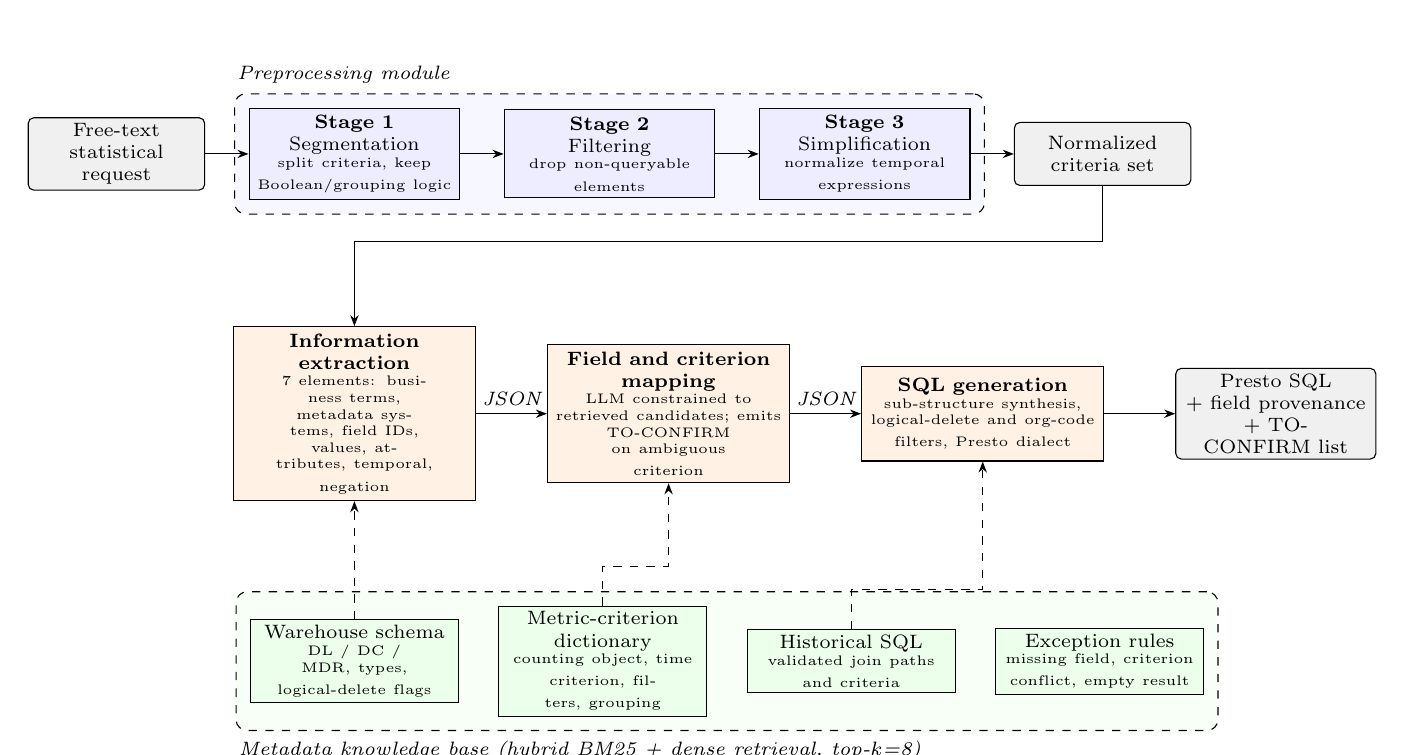
\begin{tikzpicture}[
  font=\scriptsize,
  node distance=3.2mm and 5.5mm,
  io/.style   ={draw,rounded corners=2pt,fill=gray!12,align=center,
                text width=21mm,minimum height=8mm,inner sep=2pt},
  st/.style   ={draw,fill=blue!7,align=center,text width=25mm,
                minimum height=11mm,inner sep=2.5pt},
  mod/.style  ={draw,fill=orange!10,align=center,text width=27mm,
                minimum height=12mm,inner sep=2.5pt},
  kb/.style   ={draw,fill=green!8,align=center,text width=25mm,
                minimum height=7mm,inner sep=2pt},
  lbl/.style  ={font=\scriptsize\itshape,inner sep=1pt},
  >={Stealth[length=4pt]}]

% ---------- Row 1 : preprocessing ----------
\node[io]  (req) {Free-text\\statistical request};
\node[st, right=of req] (s1) {\textbf{Stage 1}\\Segmentation\\{\tiny split criteria, keep\\Boolean/grouping logic}};
\node[st, right=of s1]  (s2) {\textbf{Stage 2}\\Filtering\\{\tiny drop non-queryable\\elements}};
\node[st, right=of s2]  (s3) {\textbf{Stage 3}\\Simplification\\{\tiny normalize temporal\\expressions}};
\node[io, right=of s3]  (norm) {Normalized\\criteria set};

\draw[->] (req)--(s1); \draw[->] (s1)--(s2); \draw[->] (s2)--(s3); \draw[->] (s3)--(norm);

\begin{scope}[on background layer]
\node[draw,dashed,rounded corners,fill=blue!3,inner sep=5pt,fit=(s1)(s2)(s3)] (pre) {};
\end{scope}
\node[lbl,anchor=south west,yshift=0.8mm] at (pre.north west) {Preprocessing module};

% ---------- Row 2 : information extraction ----------
\node[mod, below=16mm of s1.south, anchor=north, text width=29mm] (ie)
  {\textbf{Information extraction}\\{\tiny 7 elements: business terms,\\metadata systems, field IDs,\\values, attributes, temporal,\\negation}};
\node[mod, right=9mm of ie, text width=29mm] (map)
  {\textbf{Field and criterion}\\\textbf{mapping}\\{\tiny LLM constrained to\\retrieved candidates; emits\\TO-CONFIRM on ambiguous\\criterion}};
\node[mod, right=9mm of map, text width=29mm] (gen)
  {\textbf{SQL generation}\\{\tiny sub-structure synthesis,\\logical-delete and org-code\\filters, Presto dialect}};
\node[io, right=9mm of gen, text width=24mm] (out)
  {Presto SQL\\+ field provenance\\+ TO-CONFIRM list};

\draw[->] (norm.south) -- ++(0,-7mm) -| (ie.north);
\draw[->] (ie)--(map); \draw[->] (map)--(gen); \draw[->] (gen)--(out);

% ---------- Row 3 : knowledge base ----------
\node[kb, below=15mm of ie.south, anchor=north] (kb1) {Warehouse schema\\{\tiny DL / DC / MDR, types,\\logical-delete flags}};
\node[kb, right=5mm of kb1] (kb2) {Metric-criterion dictionary\\{\tiny counting object, time\\criterion, filters, grouping}};
\node[kb, right=5mm of kb2] (kb3) {Historical SQL\\{\tiny validated join paths\\and criteria}};
\node[kb, right=5mm of kb3] (kb4) {Exception rules\\{\tiny missing field, criterion\\conflict, empty result}};

\begin{scope}[on background layer]
\node[draw,dashed,rounded corners,fill=green!3,inner sep=5pt,
      fit=(kb1)(kb2)(kb3)(kb4)] (kbx) {};
\end{scope}
\node[lbl,anchor=north west,yshift=-0.8mm] at (kbx.south west)
  {Metadata knowledge base (hybrid BM25 + dense retrieval, top-$k$=8)};

\draw[->,dashed] (kb1.north) -- ++(0,5mm) -| (ie.south);
\draw[->,dashed] (kb2.north) -- ++(0,5mm) -| (map.south);
\draw[->,dashed] (kb3.north) -- ++(0,5mm) -| (gen.south);

% ---------- JSON annotation ----------
\node[lbl,above=0.6mm] at ($(ie.east)!0.5!(map.west)$)  {JSON};
\node[lbl,above=0.6mm] at ($(map.east)!0.5!(gen.west)$) {JSON};

\end{tikzpicture}
\end{figure}

\subsection{Large Language Model Configuration}
We employed gpt-4o (\PH{release date}) via API and an on-premises deployment of
qwen2.5:7b served through vLLM, with task-specific prompting strategies
optimized through iterative refinement. Zero-shot prompting was utilized for
straightforward tasks including request segmentation and criterion
classification, which minimized token usage and inference cost. Few-shot
prompting with carefully selected examples enhanced performance for complex
tasks including field and criterion mapping and SQL generation. All prompts
incorporated explicit instructions for Presto dialect compliance, mandatory
logical-deletion and organization-code filtering, and error handling. Decoding
was deterministic (temperature 0, top-$p$ 1) for all models. No patient-level
data were transmitted to any cloud endpoint; cloud models received only
de-identified metadata and synthetic values. Complete prompt templates are
provided in Table S1 in Multimedia Appendix 2.

\subsection{Comparative Evaluation Framework}

\subsubsection{Business Term Mapping Assessment}
To evaluate the performance of the LLM in mapping business terms to warehouse
fields and counting criteria, we utilized a previously constructed development
dataset comprising 30 reporting tasks across three subject domains: surgery and
anesthesia, blood transfusion, and laboratory. This dataset included diverse
expressions of statistical criteria and institutional terminology, making it
suitable for assessing mapping accuracy within the CDW. We compared the LLM with
RBFM, the field matcher currently deployed in our metadata portal. While the LLM
performs contextual natural language understanding, RBFM uses string
normalization, Levenshtein distance--based similarity scoring, and a curated
synonym table to identify candidate warehouse fields. In our experiments, RBFM
was run using its production settings, and the top-ranked field based on
similarity score was selected for each input term. Relevant business terms were
extracted from the request text of each task and mapped using both the LLM and
RBFM.

Two clinical data engineers then jointly reviewed the mapping results from both
systems and selected the most appropriate warehouse field and counting criterion
through mutual consensus. In each case, they either chose the better of the two
candidate mappings or, when necessary, manually assigned a more suitable one.
This consensus-based evaluation approach reflects real-world reporting practice
and contributes to the reliability and validity of the reference standard.

\subsubsection{SQL Query Validation}
To rigorously evaluate the accuracy and applicability of the generated SQL
queries within the CDW, we conducted an expert-based validation involving two
experts with strong proficiency in both hospital statistical criteria and the
warehouse schema. Generated SQL queries underwent systematic evaluation using 72
predefined evaluation criteria designed to assess three key dimensions: SQL
syntax adherence, warehouse schema compliance, and criteria contextual accuracy.
Each expert independently rated all applicable criteria on a 4-point scale
(1=noncompliant and 4=fully compliant), with final scores calculated as the
average of both ratings.

The evaluation framework was applied differentially based on query content. For
all generated queries, the full set of 72 criteria was used to assess structural
and schema-level accuracy. However, for queries containing business terms from
our prevalidated criterion map, only 18 criteria from the original 72 were
applicable---these specifically evaluated criterion inclusion accuracy and field
identifier correctness. Inter-rater reliability was measured using Cohen kappa,
with discrepancies resolved through consensus discussion.

This expert-driven evaluation allowed for the identification of critical
issues---such as misinterpretation of counting logic, inaccurate temporal
constraints, or improper use of DL-layer tables where a DC-layer aggregate was
required---that automated methods might overlook. As a result, we verified that
the generated SQL queries were not only technically correct but also
statistically meaningful and suitable for use in real-world hospital reporting.
The complete list of evaluation criteria is provided in Table S1 in Multimedia
Appendix 3.

\subsubsection{Statistical Result Validation}
To assess real-world performance of the automatically generated SQL queries, we
conducted result-set extraction experiments using the production CDW of
\PH{Hospital Name}. Given the resource-intensive nature of building complete
gold-standard cohorts manually, we utilized engineer-authored, criterion-
confirmed historical reference SQL as reference standards. A total of three
reporting tasks were included in this evaluation---RPT-001, RPT-002, and
RPT-005---which collectively comprised 31 statistical criteria. These tasks were
selected because validated reference SQL was available for at least one of their
criteria, allowing for meaningful comparison between system-generated result
sets and internally certified standards. Each criterion was screened based on
two conditions: (1) convertible to a single-statement Presto query and (2)
availability of a validated reference query. For these selected
criteria---including elective surgery volume and emergency surgery volume
(RPT-001), unplanned reoperation (RPT-002), and critical laboratory value
exposure (RPT-005)---SQL queries were automatically generated using our system
and executed against the production CDW.

Set similarity between system-generated and reference result sets was quantified
using two complementary set-based metrics: Jaccard index (intersection/union)
and overlap coefficient (intersection/minimum set size). The Jaccard index
provides a symmetric measure of overall similarity, while the overlap
coefficient indicates the extent to which the smaller set is contained within
the larger set, useful for identifying cases of incomplete criterion coverage.
This approach enabled objective assessment of query accuracy without requiring
manual chart review, leveraging established internal reference standards for
scalable validation. Additionally, to demonstrate technical feasibility,
successfully generated SQL queries were executed against SynHDW to assess
retrieval capabilities. Patient counts were recorded for selected tasks where
queries were executed without errors.

\subsection{Experimental Design}
Although gpt-4o was used for initial system development due to its strong
performance, the limited metadata coverage in SynHDW provided an opportunity to
systematically compare hallucination patterns across multiple LLMs, informing
optimal model selection for different reporting scenarios. The 24 tasks for the
main study included surgery and anesthesia (7 tasks), blood transfusion (5
tasks), laboratory (5 tasks), medical-record and case-mix (4 tasks), and others
(3 tasks), with complexity levels categorized as simple (10), moderate (9), and
complex (5). We employed a factorial design testing eight LLMs (three
cloud-based: gpt-4o \cite{gpt4}, deepseek-v3 \cite{dsv3}, and claude-3.5-sonnet
\cite{claude35}; five locally deployed: qwen2.5:7b \cite{qwen25}, glm4:9b
\cite{glm4}, llama3:8b \cite{llama3}, deepseek-r1:7b \cite{dsr1}, and phi3
\cite{phi3}) with five prompting
strategies (zero\_shot, structured\_approach, explicit\_uncertainty,
validation\_focused, and error\_aware). The five prompting strategies were
designed to test different approaches to query generation:

\begin{itemize}[leftmargin=1.4em,itemsep=1pt,topsep=2pt]
  \item zero\_shot: Direct query without examples or guidance
  \item structured\_approach: Step-by-step sub-structure decomposition guidance
  \item explicit\_uncertainty: Encouraging TO-CONFIRM use for uncertain criteria
  \item validation\_focused: Emphasizing validation and accuracy requirements
  \item error\_aware: Including SynHDW coverage limits and common pitfalls
\end{itemize}

\noindent Following a pilot phase (6 tasks $\times$ 8 models $\times$ 5
prompts=240 queries) for methodology validation, the main study analyzed 960
queries (24 tasks $\times$ 8 models $\times$ 5 prompts).

\subsection{Hallucination Detection and Classification}
An automated detection system was developed to identify hallucinations in
generated SQL queries. The system validated every table and column identifier
against the SynHDW metadata inventory and verified criterion appropriateness
against the metric-criterion dictionary. For the initial validation phase, we
analyzed SQL generation failures from the seven validation tasks. For the
large-scale model comparison, we developed a five-category hallucination
classification schema ordered by severity. Category A (Critical) comprised
nonexistent table or column identifiers that invalidate query results. Category
B (Major) included valid fields assigned to the wrong counting criterion---for
example, counting a monthly surgical volume by discharge time instead of room-in
time---which yields an executable query and a wrong number. Category C (Major)
captured natural language left in an identifier position, reflecting confusion
between a business term and a column name. Category D (Moderate) consisted of
placeholder values requiring manual intervention. Category E (Minor) encompassed
easily correctable dialect or schema errors, including omission of the mandatory
logical-deletion or organization-code filter. This classification specifically
evaluated model tendencies toward generating inappropriate field and criterion
references, distinct from the initial error analysis.

\subsection{Analytical Framework of Model Performance}
Model performance was evaluated across four dimensions. The model performance
dimension compared effective SQL generation rates, hallucination frequencies,
and error distributions across eight LLMs. The prompt strategy dimension
assessed five prompting approaches to identify optimal error minimization
strategies. The subject domain dimension analyzed performance variations across
surgery and anesthesia, blood transfusion, laboratory, medical-record, and
billing concepts. The complexity dimension examined correlations between query
complexity (criteria count, join depth, temporal constraints) and error
occurrence.

\subsection{Statistical Analysis}
Statistical analyses were performed using Python \PH{3.x} (Python Software
Foundation) with the scipy library (version \PH{x.x.x}) \cite{scipy2020} and
statsmodels library (version \PH{x.x.x}) \cite{statsmodels2010}. For mapping
comparisons between the LLM and RBFM, McNemar's test was applied to paired binary
outcomes \cite{mcnemar1947}. Inter-rater agreement was interpreted according to
conventional benchmarks for the kappa statistic \cite{landis1977}. Three primary performance
metrics were calculated: (1) SQL generation rate as the proportion of tasks
producing syntactically valid SQL, (2) hallucination rate as the proportion of
generated queries containing invalid field identifiers or criterion assignments,
and (3) effective SQL generation rate, calculated as SQL generation rate
$\times$ (1--hallucination rate), representing queries both syntactically valid
and free from field or criterion hallucinations.

Model performance across the eight LLMs was compared using one-way ANOVA
followed by Tukey honestly significant difference (HSD) test for post hoc
pairwise comparisons \cite{tukey1949}. Effect sizes were quantified using Cohen $d$ to assess the
practical significance of differences between prompting strategies. $\chi^2$
tests evaluated the distribution of hallucination types across models. Multiple
linear regression analysis identified predictors of hallucination rates, with
model type, prompt strategy, and query complexity as independent variables;
model fit was assessed using $R^2$. All statistical tests employed $\alpha$=.05
with Bonferroni correction for multiple comparisons where applicable.

\subsection{Ethical Considerations}
This study protocol was reviewed and approved by the Institutional Review Board
of \PH{Hospital Name} (IRB No.\ \PH{XXXX-XXXX}). As this study did not involve
prospective human participants, informed consent was waived. All data used in
the study were de-identified prior to analysis, no individual-level identifiable
information was accessed, and all model inference on real data was performed on
premises so that patient data never left the institution.

\subsection{Data and Code Availability}
Source code, including the complete pipeline implementation and hallucination
detection system, is available at \PH{repository URL}. The SynHDW generator and
its schema manifest are released with the code. De-identified metadata schemas,
the metric-criterion dictionary, and the evaluation task set are available upon
request with appropriate data use agreements, subject to institutional
data-governance constraints. Detailed documentation for system deployment and
reproduction is provided in the repository.

%==============================================================================
\section{Results}
%==============================================================================

\subsection{Preprocessing and Statistical Criteria Extraction}
Analysis of the seven validation tasks revealed substantial heterogeneity in
request complexity, ranging from 8 to 21 criteria per task (12.9$\pm$4.2). The
three-stage preprocessing pipeline systematically reduced linguistic complexity
while preserving statistical semantics (Figure~\ref{fig:preproc}). Initial
segmentation achieved modest token reduction (348.6$\pm$61.7) while maintaining
structural integrity. Subsequent filtering of non-queryable request elements
reduced both criteria count (10.4$\pm$3.5) and token count (302.9$\pm$53.6).
Final simplification yielded 9.6$\pm$3.3 criteria with 134.6$\pm$23.6 tokens per
task, representing a 61.4\% overall token reduction.

%------------------------------ FIGURE 2 ------------------------------
\begin{figure}[!t]
\caption{Progressive reduction in token count and criteria through preprocessing
stages. (A) Token count changes across segmentation, filtering, and
simplification stages for seven validation tasks. (B) Corresponding changes in
criteria count. Tasks shown are as follows: RPT-001 (monthly elective surgery
volume by department), RPT-002 (unplanned reoperation rate), RPT-003
(postanesthesia care unit throughput and delayed-discharge rate), RPT-004
(monthly blood transfusion volume and transfusion-reaction rate), RPT-005
(critical laboratory value notification timeliness), RPT-006 (surgical site
infection surveillance denominator), RPT-007 (day-surgery share of total
operative volume). Dashed black line indicates the mean across tasks.}
\label{fig:preproc}
\centering
\vspace{2pt}

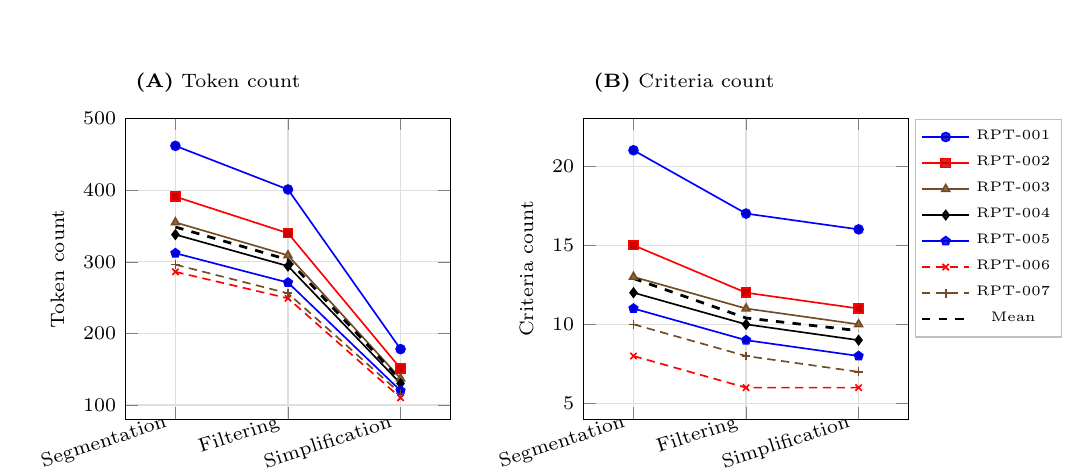
\begin{tikzpicture}
\begin{groupplot}[
  group style={group size=2 by 1, horizontal sep=17mm},
  width=0.47\linewidth, height=5.4cm,
  /tikz/font=\scriptsize,
  symbolic x coords={Segmentation,Filtering,Simplification},
  xtick=data,
  x tick label style={rotate=18,anchor=east},
  enlarge x limits=0.22,
  grid=major, grid style={gray!25},
  legend style={font=\tiny,draw=gray!50,fill=white,fill opacity=0.85,
                text opacity=1,at={(1.02,1.0)},anchor=north west,
                row sep=0.5pt,inner sep=2pt},
  every axis plot/.append style={mark size=1.6pt,line width=0.6pt},
]

%------------- Panel A : tokens -------------
\nextgroupplot[ylabel={Token count},ymin=80,ymax=500,
               title={\textbf{(A)} Token count},title style={at={(0,1)},anchor=south west,font=\scriptsize}]
\addplot+[mark=*]        coordinates {(Segmentation,462)(Filtering,401)(Simplification,178)};
\addplot+[mark=square*]  coordinates {(Segmentation,391)(Filtering,340)(Simplification,151)};
\addplot+[mark=triangle*]coordinates {(Segmentation,355)(Filtering,309)(Simplification,137)};
\addplot+[mark=diamond*] coordinates {(Segmentation,338)(Filtering,294)(Simplification,130)};
\addplot+[mark=pentagon*]coordinates {(Segmentation,312)(Filtering,271)(Simplification,120)};
\addplot+[mark=x]        coordinates {(Segmentation,286)(Filtering,249)(Simplification,110)};
\addplot+[mark=+]        coordinates {(Segmentation,296)(Filtering,256)(Simplification,116)};
\addplot[black,dashed,line width=1pt,mark=none]
  coordinates {(Segmentation,348.6)(Filtering,302.9)(Simplification,134.6)};

%------------- Panel B : criteria -------------
\nextgroupplot[ylabel={Criteria count},ymin=4,ymax=23,
               title={\textbf{(B)} Criteria count},title style={at={(0,1)},anchor=south west,font=\scriptsize}]
\addplot+[mark=*]        coordinates {(Segmentation,21)(Filtering,17)(Simplification,16)};
\addlegendentry{RPT-001}
\addplot+[mark=square*]  coordinates {(Segmentation,15)(Filtering,12)(Simplification,11)};
\addlegendentry{RPT-002}
\addplot+[mark=triangle*]coordinates {(Segmentation,13)(Filtering,11)(Simplification,10)};
\addlegendentry{RPT-003}
\addplot+[mark=diamond*] coordinates {(Segmentation,12)(Filtering,10)(Simplification,9)};
\addlegendentry{RPT-004}
\addplot+[mark=pentagon*]coordinates {(Segmentation,11)(Filtering,9)(Simplification,8)};
\addlegendentry{RPT-005}
\addplot+[mark=x]        coordinates {(Segmentation,8)(Filtering,6)(Simplification,6)};
\addlegendentry{RPT-006}
\addplot+[mark=+]        coordinates {(Segmentation,10)(Filtering,8)(Simplification,7)};
\addlegendentry{RPT-007}
\addplot[black,dashed,line width=1pt,mark=none]
  coordinates {(Segmentation,12.9)(Filtering,10.4)(Simplification,9.6)};
\addlegendentry{Mean}
\end{groupplot}
\end{tikzpicture}
\end{figure}

This preprocessing identified 67 statistical criteria suitable for automated
query generation. Information extraction from these 67 preprocessed criteria
yielded 163 unique business terms successfully mapped to warehouse-compatible
elements. Domain distribution analysis revealed that surgery and anesthesia
concepts comprised the predominant category (n=61, 37.4\%), followed by
registration and visit (n=28, 17.2\%), diagnosis and medical record (n=24,
14.7\%), laboratory (n=18, 11.0\%), blood transfusion (n=14, 8.6\%), fee and
billing (n=9, 5.5\%), staff and organization (n=6, 3.7\%), and ward and bed
(n=3, 1.8\%) domains (Table~\ref{tab:domains}). Term frequency analysis
identified time-criterion terms as the most prevalent. ``Operation room-in
time'' appeared in all 7 tasks (100.0\%; 11 mentions). Other frequent terms
included ``discharge date'' (5/7 tasks, 71.4\%; 8 mentions), ``department''
(5/7 tasks, 71.4\%; 7 mentions), ``elective surgery'' (3/7 tasks, 42.9\%; 5
mentions), ``unplanned reoperation'' (2/7 tasks, 28.6\%; 4 mentions), ``ASA
physical status classification'' (2/7 tasks, 28.6\%; 3 mentions), ``transfusion
reaction'' (2/7 tasks, 28.6\%; 3 mentions), and ``complication'' (2/7 tasks,
28.6\%; 3 mentions), as shown in Table~\ref{tab:terms}. Percentages are
calculated based on the number of tasks in which the term appeared, and mentions
indicate the number of criteria within tasks in which the term appeared.

%------------------------------ TABLE 1 ------------------------------
\begin{table}[!t]
\caption{Distribution of extracted business terms by clinical data warehouse
(CDW)\tnote{a} subject domain.}
\label{tab:domains}
\centering
\footnotesize
\begin{tabular}{@{}L{8.2cm}r@{}}
\toprule
Domains & Count (n=163), n (\%)\\
\midrule
Surgery and anesthesia        & 61 (37.4)\\
Registration and visit        & 28 (17.2)\\
Diagnosis and medical record  & 24 (14.7)\\
Laboratory                    & 18 (11.0)\\
Blood transfusion             & 14 (8.6)\\
Fee and billing               & 9 (5.5)\\
Staff and organization        & 6 (3.7)\\
Ward and bed                  & 3 (1.8)\\
\bottomrule
\end{tabular}
\tabfoot{\tnote{a}CDW: clinical data warehouse.}
\end{table}

%------------------------------ TABLE 2 ------------------------------
\begin{table}[!t]
\caption{Ten most frequently occurring business terms across all tasks.}
\label{tab:terms}
\centering
\footnotesize
\begin{tabular}{@{}L{7.0cm}rr@{}}
\toprule
Business terms & Tasks (n=7), n (\%) & Mentions (criterion), n\\
\midrule
Operation room-in time                 & 7 (100.0) & 11\\
Discharge date                         & 5 (71.4)  & 8\\
Department                             & 5 (71.4)  & 7\\
Elective surgery                       & 3 (42.9)  & 5\\
Unplanned reoperation                  & 2 (28.6)  & 4\\
ASA\tnote{a} physical status classification & 2 (28.6) & 3\\
Transfusion reaction                   & 2 (28.6)  & 3\\
Complication                           & 2 (28.6)  & 3\\
PACU\tnote{b} discharge time           & 1 (14.3)  & 2\\
Critical laboratory value              & 1 (14.3)  & 2\\
\bottomrule
\end{tabular}
\tabfoot{\tnote{a}ASA: American Society of Anesthesiologists.\\
\tnote{b}PACU: postanesthesia care unit.}
\end{table}

\subsection{Comparative Performance of Mapping Approaches}
Evaluation of mapping accuracy demonstrated the LLM's superior performance
compared to RBFM across 412 business terms extracted from the 30 development
tasks. The LLM achieved an overall accuracy of 53.9\% (222/412) versus RBFM's
34.5\% (142/412), a statistically significant difference ($P<.001$, McNemar's
test). Domain-stratified analysis revealed the LLM's highest accuracy in the
surgery and anesthesia domain (71.8\%, 61/85) and lowest in the laboratory
domain (36.7\%, 33/90), suggesting particular challenges with test-item concepts
requiring numeric threshold and unit interpretation.

Notably, among the 270 terms that RBFM misclassified, the LLM correctly mapped
79 (29.3\%), demonstrating superior contextual understanding. For instance, RBFM
incorrectly mapped ``operation room-in time'' to the admission timestamp on the
registration table---a lexically close but semantically different field---while
the LLM correctly identified the room-in timestamp on the anesthesia record.
This pattern of improved semantic interpretation was consistent across
multiword, criterion-bearing terms.

\subsection{SQL Query Generation Quality and Expert Validation}
Two domain experts independently evaluated SQL queries generated from the seven
validation tasks using 72 predefined criteria across three dimensions: SQL
syntax adherence, warehouse schema compliance, and criteria contextual accuracy
(inter-rater reliability: Cohen $\kappa$=0.87). Each criterion was rated on a
4-point scale (1=noncompliant and 4=fully compliant). SQL syntax adherence
achieved near-perfect scores from expert reviewers (3.96$\pm$0.14) and matched
LLM self-evaluation (4.00$\pm$0.00), confirming robust syntactic generation
capabilities. Warehouse schema compliance similarly demonstrated strong
performance (expert: 3.85$\pm$0.23, LLM: 4.00$\pm$0.00), indicating successful
adaptation to the layered table structures and their join paths.

However, criteria contextual accuracy exhibited greater variability and lower
absolute scores (expert: 3.08$\pm$0.51, LLM: 3.49$\pm$0.34), with the
0.41-point difference suggesting systematic LLM overconfidence in criterion
interpretation ($P$=.017, paired $t$ test). This divergence was most pronounced
for criteria involving temporal choices or multicondition counting logic.

Among the total queries evaluated, 24 contained prevalidated criteria from our
development dataset, enabling additional validation of mapping accuracy. For
these queries, criterion inclusion accuracy averaged 3.38$\pm$0.41 (expert)
versus 3.52$\pm$0.31 (LLM), while field identifier correctness achieved higher
scores of 3.74$\pm$0.26 (expert) versus a perfect score of 4.00$\pm$0.00 (LLM).
The perfect LLM score for field identifier correctness reflects its consistent
ability to generate syntactically valid identifiers, though not necessarily
criterion-appropriate ones.

\subsection{Statistical Result Retrieval Performance}
Validation using engineer-certified reference SQL revealed that performance
strongly correlated with criterion complexity (Table~\ref{tab:retrieval}). For
the three evaluated tasks (RPT-001, RPT-002, and RPT-005), we assessed four
distinct statistical criteria that had available reference standards. The query
for elective surgery volume (RPT-001) demonstrated high retrieval accuracy,
achieving a Jaccard index of 0.86 and a perfect overlap coefficient of 1.0,
indicating that the system-generated result set closely matched the reference
set. In contrast, emergency surgery volume showed a very low Jaccard index of
0.05 despite an overlap coefficient of 1.0, suggesting that while the retrieved
cases were all contained in the reference set, a large portion of the reference
cases was not captured---traced to the model filtering on a single emergency
flag rather than the institution's two-flag definition. The unplanned
reoperation criterion (RPT-002) resulted in complete retrieval failure, with
both the Jaccard index and overlap coefficient equal to 0, indicating that no
matching cases were retrieved. This reflects the system's selection of a
structurally plausible planning flag that is unpopulated throughout the
warehouse, rather than the reoperation marker actually used by the surgical
application table---a failure mode invisible to syntax and schema checking. The
critical laboratory value exposure criterion (RPT-005) achieved moderate
performance, with a Jaccard index of 0.22 and an overlap coefficient of 0.51,
reflecting partial mapping success for an indicator represented by a mix of
numeric thresholds and notification records.

%------------------------------ TABLE 3 ------------------------------
\begin{table}[!t]
\caption{Comparison of result-set retrieval between system-generated queries and
validated reference SQL\tnote{a}.}
\label{tab:retrieval}
\centering
\footnotesize
\begin{tabular}{@{}L{2.0cm}L{5.4cm}rr@{}}
\toprule
Task ID & Simplified criterion & Jaccard similarity & Overlap coefficient\\
\midrule
RPT-002 & Unplanned reoperation                & 0    & 0\\
RPT-001 & Emergency surgery volume             & 0.05 & 1.0\\
        & Elective surgery volume              & 0.86 & 1.0\\
RPT-005 & Critical laboratory value exposure   & 0.22 & 0.51\\
\bottomrule
\end{tabular}
\tabfoot{\tnote{a}SQL: Structured Query Language.}
\end{table}

These results collectively highlight that the system is capable of achieving
high performance when querying well-defined, single-criterion indicators (eg,
elective surgery volume) but may underperform when indicator definitions are
compound, institution-specific, or depend on fields whose population is
incomplete (eg, emergency surgery volume or unplanned reoperation). Improvements
in criterion dictionary coverage and field-population profiling may be necessary
to enhance retrieval for more complex statistical criteria.

\subsection{Large-Scale Model Comparison and Hallucination Analysis}
To systematically evaluate hallucination patterns across multiple LLMs, we
conducted a separate large-scale experiment using SynHDW, analyzing 960 SQL
generation attempts (24 reporting tasks $\times$ 8 models $\times$ 5 prompting
strategies), distinct from our initial validation study. Analysis of 960 SQL
generation attempts revealed significant heterogeneity in model performance
($F_{7,799}$=3.72, $P<.001$), with hallucination rates ranging from 19.5\%
(n=21) to 47.1\% (n=50) among models achieving $>$80\% SQL generation success.
The overall hallucination rate was 32.6\% (n=263) (95\% CI 29.4\%--35.9\%), with
substantial variation in both generation capability and accuracy across models
(Figure~\ref{fig:models} and Table~\ref{tab:modelperf}).

%------------------------------ FIGURE 3 ------------------------------
\begin{figure}[!t]
\caption{Comprehensive performance analysis of eight large language models for
clinical data warehouse (CDW) Structured Query Language (SQL) generation. (A)
Comparison of hallucination rates and effective SQL rates across models. (B)
Cost-performance trade-off analysis showing the relationship between cost per
query (log scale) and effective SQL rate, with bubble size proportional to
effective rate. Cloud models (blue) and on-premises models (orange) show
distinct clustering patterns. On-premises models incur no per-query API charge;
they are plotted at their amortized cost, computed as inference time $\times$
US~\$0.30 per GPU-hour under the institution's 3-year hardware amortization.}
\label{fig:models}
\centering
\vspace{2pt}

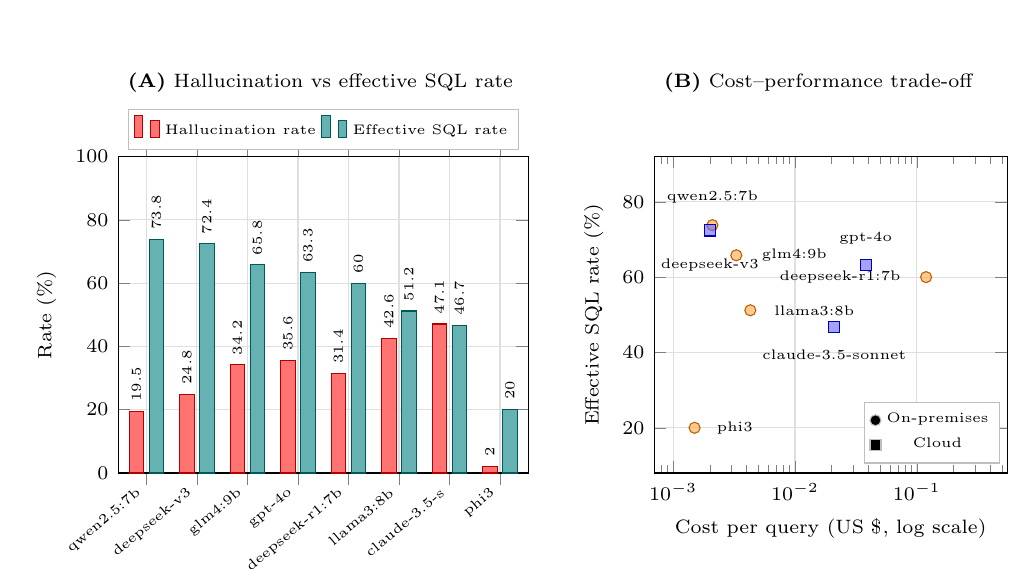
\begin{tikzpicture}
%------------- Panel A -------------
\begin{axis}[
  name=panelA,
  width=0.56\linewidth, height=5.6cm, font=\scriptsize,
  ybar, bar width=5.2pt,
  symbolic x coords={qwen2.5:7b,deepseek-v3,glm4:9b,gpt-4o,deepseek-r1:7b,
                     llama3:8b,claude-3.5-s,phi3},
  xtick=data, x tick label style={rotate=40,anchor=east,font=\tiny},
  ymin=0, ymax=100, ylabel={Rate (\%)},
  grid=major, grid style={gray!25},
  legend style={font=\tiny,at={(0.5,1.02)},anchor=south,legend columns=2,
                draw=gray!50,inner sep=2pt},
  enlarge x limits=0.08,
  nodes near coords, every node near coord/.append style={font=\tiny,rotate=90,anchor=west},
  title={\textbf{(A)} Hallucination vs effective SQL rate},
  title style={at={(0,1.12)},anchor=south west,font=\scriptsize},
]
\addplot[fill=red!55,draw=red!70!black] coordinates {
  (qwen2.5:7b,19.5) (deepseek-v3,24.8) (glm4:9b,34.2) (gpt-4o,35.6)
  (deepseek-r1:7b,31.4) (llama3:8b,42.6) (claude-3.5-s,47.1) (phi3,2.0)};
\addlegendentry{Hallucination rate}
\addplot[fill=teal!60,draw=teal!70!black] coordinates {
  (qwen2.5:7b,73.8) (deepseek-v3,72.4) (glm4:9b,65.8) (gpt-4o,63.3)
  (deepseek-r1:7b,60.0) (llama3:8b,51.2) (claude-3.5-s,46.7) (phi3,20.0)};
\addlegendentry{Effective SQL rate}
\end{axis}

%------------- Panel B -------------
\begin{axis}[
  name=panelB, at={($(panelA.east)+(16mm,0)$)}, anchor=west,
  width=0.50\linewidth, height=5.6cm, font=\scriptsize,
  xmode=log, log basis x=10,
  xlabel={Cost per query (US \$, log scale)},
  ylabel={Effective SQL rate (\%)},
  xmin=0.0007, xmax=0.55, ymin=8, ymax=92,
  grid=major, grid style={gray!25},
  legend style={font=\tiny,at={(0.98,0.03)},anchor=south east,draw=gray!50,inner sep=2pt},
  title={\textbf{(B)} Cost--performance trade-off},
  title style={at={(0,1.12)},anchor=south west,font=\scriptsize},
]
% on-premises models (orange)
\addplot[scatter, only marks, mark=*,
         visualization depends on={\thisrow{sz} \as \perpointmarksize},
         scatter/@pre marker code/.append style={/tikz/mark size=\perpointmarksize},
         scatter/use mapped color={draw=orange!75!black,fill=orange!70,fill opacity=0.60}]
  table[x=x,y=y] {
x        y     sz
0.0021   73.8  6.6
0.0033   65.8  5.4
0.1190   60.0  4.7
0.0043   51.2  3.6
0.0015   20.0  1.4
};
\addlegendentry{On-premises}
% cloud models (blue)
\addplot[scatter, only marks, mark=square*,
         visualization depends on={\thisrow{sz} \as \perpointmarksize},
         scatter/@pre marker code/.append style={/tikz/mark size=\perpointmarksize},
         scatter/use mapped color={draw=blue!70!black,fill=blue!60,fill opacity=0.60}]
  table[x=x,y=y] {
x        y     sz
0.0020   72.4  6.4
0.0210   46.7  3.2
0.0380   63.3  5.2
};
\addlegendentry{Cloud}
% annotations (placed to avoid mutual overlap and axis-edge clipping)
\node[font=\tiny,anchor=south,yshift=1.6mm]      at (axis cs:0.0021,73.8) {qwen2.5:7b};
\node[font=\tiny,anchor=north,yshift=-2.4mm]     at (axis cs:0.0020,72.4) {deepseek-v3};
\node[font=\tiny,anchor=south,yshift=1.4mm]      at (axis cs:0.0380,63.3) {gpt-4o};
\node[font=\tiny,anchor=west,xshift=2.0mm]       at (axis cs:0.0033,65.8) {glm4:9b};
\node[font=\tiny,anchor=east,xshift=-2.0mm]      at (axis cs:0.1190,60.0) {deepseek-r1:7b};
\node[font=\tiny,anchor=west,xshift=1.8mm]       at (axis cs:0.0043,51.2) {llama3:8b};
\node[font=\tiny,anchor=north,yshift=-1.6mm]     at (axis cs:0.0210,46.7) {claude-3.5-sonnet};
\node[font=\tiny,anchor=west,xshift=1.6mm]       at (axis cs:0.0015,20.0) {phi3};
\end{axis}
\end{tikzpicture}
\end{figure}

%------------------------------ TABLE 4 ------------------------------
\begin{table}[!t]
\caption{Model performance summary.}
\label{tab:modelperf}
\centering
\footnotesize
\setlength{\tabcolsep}{4pt}
\begin{tabular}{@{}L{2.5cm}L{1.5cm}C{1.5cm}C{1.6cm}C{1.5cm}C{1.9cm}C{1.5cm}@{}}
\toprule
Model & Architecture & SQL\tnote{a} generation (\%) & Hallucination (\%)\tnote{b}
      & Effective SQL (\%)\tnote{c} & Time (s)\tnote{d} & Cost (US \$)/Query\\
\midrule
qwen2.5:7b        & On-premises & 91.7  & 19.5          & 73.8 & 24.6$\pm$5.8      & 0.000\\
deepseek-v3       & Cloud       & 96.3  & 24.8          & 72.4 & 8.4$\pm$2.1       & 0.002\\
glm4:9b           & On-premises & 100.0 & 34.2          & 65.8 & 39.4$\pm$9.7      & 0.000\\
gpt-4o            & Cloud       & 98.3  & 35.6          & 63.3 & 19.7$\pm$4.8      & 0.038\\
deepseek-r1:7b    & On-premises & 87.5  & 31.4          & 60.0 & 1428.6$\pm$377.2  & 0.000\\
llama3:8b         & On-premises & 89.2  & 42.6          & 51.2 & 52.1$\pm$13.4     & 0.000\\
claude-3.5-sonnet & Cloud       & 88.3  & 47.1          & 46.7 & 15.2$\pm$3.9      & 0.021\\
phi3              & On-premises & 20.4  & 2.0\tnote{e}  & 20.0 & 18.3$\pm$7.6      & 0.000\\
\bottomrule
\end{tabular}
\tabfoot{\tnote{a}SQL: Structured Query Language.\\
\tnote{b}Percentage of generated queries with invalid field identifiers or
criterion assignments.\\
\tnote{c}SQL generation $\times$ (1--hallucination).\\
\tnote{d}Mean$\pm$SD.\\
\tnote{e}Misleading due to low generation rate.}
\end{table}

Qwen2.5:7b emerged as the most effective model with a 73.8\% effective SQL rate
despite moderate SQL generation capability (91.7\%), attributed to its low
hallucination rate (19.5\%) and minimal placeholder usage (28.6\%). In contrast,
gpt-4o showed high SQL generation (98.3\%) but a lower effective rate (63.3\%)
due to heavy placeholder usage (35.7\%) and a marked tendency to substitute a
plausible timestamp when the requested counting criterion was not explicit.

\subsection{Hallucination Pattern Analysis}
Classification of 263 hallucinations revealed distinct error patterns across
models (Figure~\ref{fig:halluc}). Category B errors (wrong criterion
assignments) predominated (34.6\%, n=91), followed by Category D (placeholder
insertions, 29.7\%, n=78) and Category E (schema and dialect errors, 24.3\%,
n=64). Category A (nonexistent field identifiers) was relatively rare (9.1\%,
n=24), as was Category C (natural language substitution, 2.3\%, n=6). $\chi^2$
analysis confirmed significant variation in error distribution across models
($\chi^2$=52.7, $df$=28, $P$=.003).

%------------------------------ FIGURE 4 ------------------------------
\begin{figure}[!t]
\caption{Distribution and analysis of hallucination types by model. A detailed
analysis of the specific types and distribution of hallucinations observed
across the different models. (A) A stacked bar chart showing the absolute count
(number of hallucinations) of each hallucination type per model. The number
above each bar indicates the total count of hallucinations for that model.
Hallucination types are classified as Type A (nonexistent field identifiers),
Type B (wrong criterion assignment), Type C (natural language in identifier
position), Type D (placeholder usage), and Type E (schema and dialect errors).
(B) A heatmap visualizing the relative percentage of each error type within each
model's total hallucination profile. The color intensity corresponds to the
percentage value, with darker shades indicating a higher proportion of that
hallucination type. The scale is provided by the color bar on the right.}
\label{fig:halluc}
\centering
\vspace{2pt}

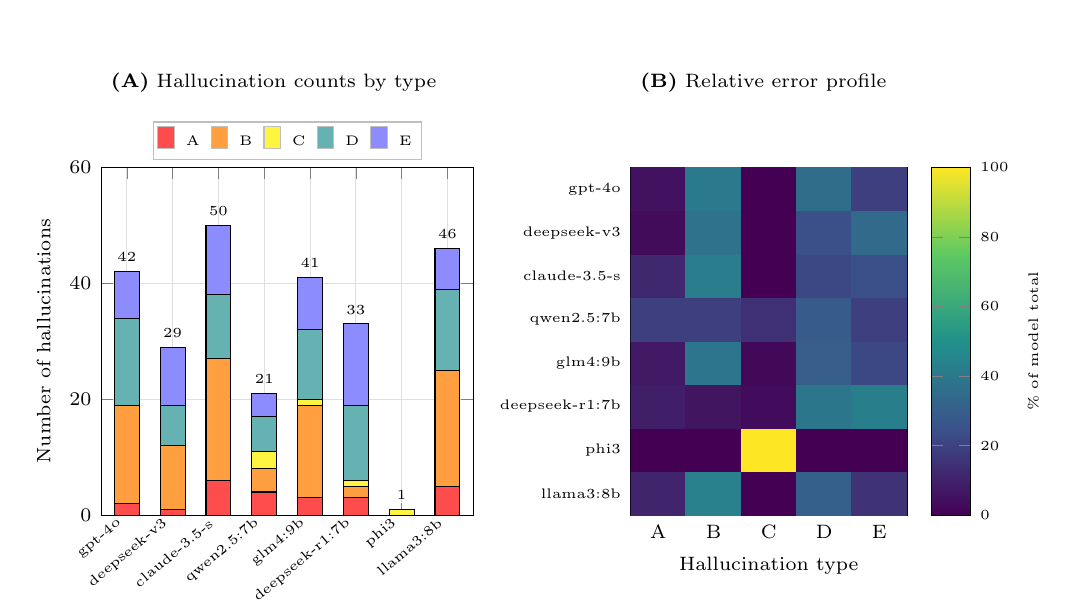
\begin{tikzpicture}
%------------- Panel A : stacked bars -------------
\begin{axis}[
  name=hA,
  width=0.52\linewidth, height=6.0cm, font=\scriptsize,
  ybar stacked, bar width=9pt,
  symbolic x coords={gpt-4o,deepseek-v3,claude-3.5-s,qwen2.5:7b,glm4:9b,
                     deepseek-r1:7b,phi3,llama3:8b},
  xtick=data, x tick label style={rotate=40,anchor=east,font=\tiny},
  ymin=0, ymax=60, ylabel={Number of hallucinations},
  grid=major, grid style={gray!25},
  legend style={font=\tiny,at={(0.5,1.02)},anchor=south,legend columns=5,
                draw=gray!50,inner sep=1.5pt,column sep=2pt},
  enlarge x limits=0.08,
  title={\textbf{(A)} Hallucination counts by type},
  title style={at={(0,1.14)},anchor=south west,font=\scriptsize},
]
\addplot[fill=red!70]     coordinates {(gpt-4o,2)(deepseek-v3,1)(claude-3.5-s,6)(qwen2.5:7b,4)(glm4:9b,3)(deepseek-r1:7b,3)(phi3,0)(llama3:8b,5)};
\addlegendentry{A}
\addplot[fill=orange!75]  coordinates {(gpt-4o,17)(deepseek-v3,11)(claude-3.5-s,21)(qwen2.5:7b,4)(glm4:9b,16)(deepseek-r1:7b,2)(phi3,0)(llama3:8b,20)};
\addlegendentry{B}
\addplot[fill=yellow!75]  coordinates {(gpt-4o,0)(deepseek-v3,0)(claude-3.5-s,0)(qwen2.5:7b,3)(glm4:9b,1)(deepseek-r1:7b,1)(phi3,1)(llama3:8b,0)};
\addlegendentry{C}
\addplot[fill=teal!60]    coordinates {(gpt-4o,15)(deepseek-v3,7)(claude-3.5-s,11)(qwen2.5:7b,6)(glm4:9b,12)(deepseek-r1:7b,13)(phi3,0)(llama3:8b,14)};
\addlegendentry{D}
\addplot[fill=blue!45]    coordinates {(gpt-4o,8)(deepseek-v3,10)(claude-3.5-s,12)(qwen2.5:7b,4)(glm4:9b,9)(deepseek-r1:7b,14)(phi3,0)(llama3:8b,7)};
\addlegendentry{E}
% totals above bars
\node[font=\tiny,anchor=south] at (axis cs:gpt-4o,42) {42};
\node[font=\tiny,anchor=south] at (axis cs:deepseek-v3,29) {29};
\node[font=\tiny,anchor=south] at (axis cs:claude-3.5-s,50) {50};
\node[font=\tiny,anchor=south] at (axis cs:qwen2.5:7b,21) {21};
\node[font=\tiny,anchor=south] at (axis cs:glm4:9b,41) {41};
\node[font=\tiny,anchor=south] at (axis cs:deepseek-r1:7b,33) {33};
\node[font=\tiny,anchor=south] at (axis cs:phi3,1) {1};
\node[font=\tiny,anchor=south] at (axis cs:llama3:8b,46) {46};
\end{axis}

%------------- Panel B : heatmap -------------
\begin{axis}[
  name=hB, at={($(hA.east)+(20mm,0)$)}, anchor=west,
  width=0.42\linewidth, height=6.0cm, font=\scriptsize,
  colormap={vlike}{rgb255=(68,1,84) rgb255=(59,82,139) rgb255=(33,145,140)
                   rgb255=(94,201,98) rgb255=(253,231,37)},
  colorbar,
  colorbar style={font=\tiny,ylabel={\% of model total},ylabel style={font=\tiny}},
  point meta min=0, point meta max=100,
  xtick={0,1,2,3,4}, xticklabels={A,B,C,D,E},
  ytick={0,1,2,3,4,5,6,7},
  yticklabels={llama3:8b,phi3,deepseek-r1:7b,glm4:9b,qwen2.5:7b,
               claude-3.5-s,deepseek-v3,gpt-4o},
  y tick label style={font=\tiny},
  xlabel={Hallucination type},
  enlarge x limits=false, enlarge y limits=false,
  title={\textbf{(B)} Relative error profile},
  title style={at={(0,1.14)},anchor=south west,font=\scriptsize},
]
\addplot[matrix plot*, point meta=explicit, mesh/cols=5] table[meta=v] {
x y v
0 0 10.9
1 0 43.5
2 0 0.0
3 0 30.4
4 0 15.2
0 1 0.0
1 1 0.0
2 1 100.0
3 1 0.0
4 1 0.0
0 2 9.1
1 2 6.1
2 2 3.0
3 2 39.4
4 2 42.4
0 3 7.3
1 3 39.0
2 3 2.4
3 3 29.3
4 3 22.0
0 4 19.0
1 4 19.0
2 4 14.3
3 4 28.6
4 4 19.0
0 5 12.0
1 5 42.0
2 5 0.0
3 5 22.0
4 5 24.0
0 6 3.4
1 6 37.9
2 6 0.0
3 6 24.1
4 6 34.5
0 7 4.8
1 7 40.5
2 7 0.0
3 7 35.7
4 7 19.0
};
\end{axis}
\end{tikzpicture}
\end{figure}

Model-specific analysis revealed distinctive failure modes
(Table~\ref{tab:halluctypes}). Claude-3.5-sonnet exhibited the highest baseline
hallucination rate (47.1\%) but showed dramatic improvement with error-aware
prompting (16.4\% hallucination and 65.2\% relative reduction). Deepseek-v3
achieved perfect accuracy (0\% hallucination) with explicit\_uncertainty
prompting, though limited to simple single-table counting queries. Phi3's
apparently low hallucination rate (2.0\%) was misleading, resulting from 79.6\%
failure to generate any SQL rather than accurate generation.

%------------------------------ TABLE 5 ------------------------------
\begin{table}[!t]
\caption{Detailed hallucination type distribution by model.}
\label{tab:halluctypes}
\centering
\footnotesize
\setlength{\tabcolsep}{3pt}
\begin{tabular}{@{}L{2.3cm}C{1.35cm}C{1.5cm}C{1.5cm}C{1.5cm}C{1.4cm}C{1.4cm}@{}}
\toprule
Model & Total halluci\-nations & Category A (nonexis\-tent), n (\%)
      & Category B (wrong criterion), n (\%)
      & Category C (natural language), n (\%)
      & Category D (place\-holder), n (\%)
      & Category E (schema errors), n (\%)\\
\midrule
gpt-4o            & 42 & 2 (4.8)  & 17 (40.5) & 0 (0)     & 15 (35.7) & 8 (19.0)\\
deepseek-v3       & 29 & 1 (3.4)  & 11 (37.9) & 0 (0)     & 7 (24.1)  & 10 (34.5)\\
claude-3.5-sonnet & 50 & 6 (12.0) & 21 (42.0) & 0 (0)     & 11 (22.0) & 12 (24.0)\\
qwen2.5:7b        & 21 & 4 (19.0) & 4 (19.0)  & 3 (14.3)  & 6 (28.6)  & 4 (19.0)\\
glm4:9b           & 41 & 3 (7.3)  & 16 (39.0) & 1 (2.4)   & 12 (29.3) & 9 (22.0)\\
deepseek-r1:7b    & 33 & 3 (9.1)  & 2 (6.1)   & 1 (3.0)   & 13 (39.4) & 14 (42.4)\\
phi3              & 1  & 0 (0)    & 0 (0)     & 1 (100)   & 0 (0)     & 0 (0)\\
llama3:8b         & 46 & 5 (10.9) & 20 (43.5) & 0 (0)     & 14 (30.4) & 7 (15.2)\\
\bottomrule
\end{tabular}
\end{table}

Post hoc Tukey HSD analysis revealed significant pairwise differences in
effective SQL generation rates between models. Qwen2.5:7b significantly
outperformed gpt-4o (mean difference=10.5\%, $P$=.03), with a medium-to-large
effect size (Cohen $d$=0.68). The performance gap between the best (qwen2.5:7b)
and worst (phi3) models was substantial ($d$=2.94), indicating practically
meaningful differences beyond statistical significance.

\subsection{Prompt Engineering Impact}
Evaluation of prompt strategies revealed substantial effect sizes (Cohen
$d>$1.0) compared to the zero\_shot baseline across all alternative strategies.
Despite these large effects, high variance in model--prompt interactions
prevented detection of a significant main effect ($F_{4,955}$=1.72, $P$=.144).
The error\_aware strategy, which explicitly acknowledged SynHDW coverage limits
and common pitfalls, proved most effective for high-hallucination models, while
explicit\_uncertainty excelled for simpler queries requiring conservative
interpretation.

\subsection{Prompt Strategy Performance Analysis}
Comprehensive analysis of prompting strategies across all 8 models (192 queries
per prompt type) revealed unexpected patterns in hallucination control. The
zero\_shot approach demonstrated superior performance with the lowest
hallucination rate (mean 15.2\%, SD 12.1\%) and highest effective SQL rate (mean
69.8\%, SD 20.7\%), significantly outperforming more complex strategies. In
contrast, structured\_approach, which provided detailed step-by-step
sub-structure guidance, showed the highest hallucination rate (mean 42.1\%, SD
24.6\%) and lowest effectiveness (mean 44.2\%, SD 19.3\%). The
validation\_focused strategy, designed to emphasize accuracy, paradoxically
decreased performance compared to zero\_shot ($P$=.038, Tukey HSD), achieving a
mean (SD) effective SQL rate of only 55.4\% (21.8\%). These findings suggest
that excessive instructional complexity may introduce confusion rather than
clarity in LLM-based SQL generation over a layered warehouse schema.

The substantial standard deviations across all metrics (ranging from 12.1\% to
26.9\%) indicate significant model-dependent variability in prompt
responsiveness. For instance, with zero\_shot prompting, deepseek-r1:7b achieved
0\% hallucination while claude-3.5-sonnet exhibited 38.2\%, representing a 38.2
percentage point difference for identical prompting. This variability was
further confirmed by regression analysis, which revealed that model architecture
explained 69\% of performance variance ($R^2$=0.69, $P<.001$), while prompt
strategy contributed marginally. Based on these findings, optimal model--prompt
combinations were identified: qwen2.5:7b with zero\_shot achieved an 82.5\%
effective SQL rate, while deepseek-v3 with explicit\_uncertainty reached 100\%
effectiveness on simple single-table counting queries, though with limited
applicability to criterion-sensitive indicators.

\subsection{Synthetic Data Validation}
To assess the practical viability of generated SQL queries, we executed
successfully generated queries against the SynHDW synthetic dataset containing
128,470 patient records. The system successfully matched 9213 synthetic patients
across two validated reporting tasks: RPT-001 (monthly elective surgery volume)
matched 3186 patients (2.5\% of dataset), while RPT-004 (monthly blood
transfusion volume) matched 6027 patients (4.7\% of dataset). These result-set
sizes are consistent with the monthly volumes observed in production reporting,
demonstrating technical feasibility, though we acknowledge that synthetic data
validation may overestimate real-world performance due to the absence of data
quality issues inherent in actual hospital systems, such as missing values,
retrospectively corrected timestamps, and coding variations across campuses.

%==============================================================================
\section{Discussion}
%==============================================================================

\subsection{Principal Findings}
We developed a comprehensive framework that automates the transformation of
free-text hospital statistical requests into Presto SQL queries over a
three-layer CDW. While initially developed with gpt-4o, our systematic
evaluation across eight LLMs revealed unexpected findings: the on-premises
qwen2.5:7b model achieved the highest effective SQL generation rate (73.8\%)
compared to gpt-4o's 63.3\%, primarily due to lower hallucination rates (19.5\%
vs 35.6\%). This counterintuitive result---where a smaller, locally hosted model
outperformed a state-of-the-art commercial model---highlights the critical
importance of hallucination control over raw generation capability in clinical
applications, and it resolves rather than sharpens the privacy--performance
tension: the deployment that keeps patient data inside the institution was also
the most accurate. Our framework successfully demonstrated a 53.9\% mapping
accuracy, significantly exceeding the 34.5\% achieved by the rule-based matcher
currently in production ($P<.001$), though performance varied substantially
across subject domains (surgery and anesthesia: 71.8\%, laboratory: 36.7\%).

This end-to-end automation represents a significant advancement over our
previous practice, though our results reveal both capabilities and limitations.
While the deployed rule-based matcher supports engineers with candidate fields
and still requires manual SQL construction, our system automates the entire
pipeline. However, our result-set validation exposed critical challenges:
complete failure in the unplanned-reoperation query (Jaccard=0.00) due to
selection of a structurally valid but unpopulated planning flag, and minimal
overlap in emergency surgery volume (Jaccard=0.05) from an incomplete
institutional flag definition. These failures, affecting half of the evaluated
criteria, underscore that despite advances in language understanding, hospital
data complexities---particularly field population and institution-specific
compound definitions---remain significant obstacles.

Through the processes of segmentation, filtering, and simplification, the
framework successfully produced structured inputs that reduced redundancy while
preserving statistical relevance. The LLM accurately identified business terms
such as procedures, laboratory items, and blood products and mapped them to
warehouse-standardized fields, thereby enhancing consistency and reusability
across reports. However, ambiguous expressions and compound
indicators---such as ``complication rate after major surgery''---sometimes led
to incorrect mappings, indicating that expert validation remains necessary in
certain cases.

The LLM was able to generate syntactically correct and executable SQL queries
based on the warehouse schema. Composition of inclusion criteria using
INTERSECT and exclusion criteria using EXCEPT or NOT IN enabled the automated
construction of denominator and numerator definitions. Nevertheless, challenges
were observed when criteria involved temporal constraints or context-dependent
conditions, often resulting in omissions or logical misinterpretations. In
addition, expansion over the DL layer when a DC-layer aggregate was available
sometimes led to increased query execution times, especially for multi-campus
tables that require organization-code filtering.

\subsection{Complementary Evaluation Strategy}
Our dual evaluation approach, combining expert assessment with quantitative
synthetic data validation, provides a more comprehensive characterization of
system performance than either method alone could achieve; we report it following
the MI-CLAIM checklist for clinical AI modeling and its generative extension
MI-CLAIM-GEN \cite{miclaim2020,miclaimgen2024}, and we state the resulting threats
to construct validity explicitly rather than by omission \cite{validity2023}.
Expert evaluation
ensures statistical meaningfulness and safety, confirming that generated queries
align with reporting intent and follow the institution's counting rules.
Synthetic validation contributes scalable, reproducible metrics that quantify
technical accuracy and identify systematic errors. This complementary strategy
revealed technical issues invisible to manual review, such as subtle type
coercions on the all-VARCHAR warehouse columns and missing logical-deletion
filters that appeared structurally correct but would silently inflate counts.
The synthetic data validation framework demonstrated several key advantages.
Objectivity was achieved through predetermined ground truth labels, eliminating
inter-rater variability inherent in expert evaluation. Scalability allowed us to
validate hundreds of thousands of rows in seconds rather than the hours required
for manual review. Reproducibility was ensured through seed-based generation,
enabling other teams to replicate our exact validation scenarios. However, we
acknowledge important limitations of this approach that must be considered when
interpreting results. The controlled nature of synthetic data, while enabling
clean performance metrics, does not fully capture real-world complexity.
Production hospital tables contain missing values, retrospectively corrected
timestamps, and campus-level coding differences that our synthetic data lacks.
We anticipate that these factors could reduce real-world performance by
\PH{XX}\%--\PH{XX}\% compared to our synthetic validation results. SynHDW's
focus on the surgical, transfusion, and laboratory subject areas also limits
validation of pathology, physical examination, and insurance-audit reporting,
important considerations for comprehensive system evaluation. Compound-indicator
scenarios presented particular challenges, as evidenced by our emergency surgery
retrieval, achieving minimal overlap (Jaccard=0.05) due to an incomplete
institutional flag definition. Criteria involving free-text clinical narrative,
such as complication descriptions recorded outside coded fields, remain untested
because they are absent from the structured warehouse. These limitations
highlight the need for continued validation using diverse subject areas and
reporting scenarios.

\subsection{Cost-Effectiveness and Scalability}
Economic feasibility remains crucial for real-world implementation of AI-powered
hospital reporting systems. Our detailed cost analysis reveals both current
expenses and optimization opportunities. At current pricing, gpt-4o API calls
average US~\$0.03--0.05 per query, with each reporting task requiring
approximately five API calls for complete processing. This translates to roughly
US~\$0.15--0.25 per task using gpt-4o. Deepseek-v3 offers substantial cost
reduction at US~\$0.002--0.004 per query, achieving over 90\% savings with
comparable performance for many use cases. For hospital-scale deployment, we
project monthly costs based on typical request volumes. Our institution
processes approximately \PH{X000} statistical requests monthly, which would
incur US~\$\PH{XXX}--\PH{XXX} using gpt-4o or US~\$\PH{XX}--\PH{XX} with
deepseek-v3. These costs compare favorably to manual authoring, which typically
requires \PH{X}--\PH{X} hours of engineer time per task. Our system processes
each task in under 2 minutes for the cloud and on-premises models other than
deepseek-r1:7b, representing time savings of \PH{XX}\%--\PH{XX}\% compared to
manual methods. Notably, the on-premises deployment that achieved the best
accuracy also carries no per-query charge; its amortized cost is dominated by
inference time, which is why the reasoning-oriented deepseek-r1:7b is the cost
outlier in Figure~\ref{fig:models}B despite running on owned hardware.

To situate our contributions within the rapidly evolving field of LLM-based
clinical data access, we compare our framework with three representative
approaches, highlighting their limitations and the necessity of our approach.
Benchmark-oriented text-to-SQL systems achieve strong execution accuracy on
public datasets but assume a small, static schema and provide no mechanism for
institution-specific counting criteria, so they cannot be transferred to a
hospital warehouse without re-engineering
\cite{yu2018,guo2019,bogin2019,tsqlsurvey2024}. Reliability-oriented EHR
text-to-SQL evaluation introduces abstention on unanswerable questions, a
property we adopt as the TO-CONFIRM behavior, but it does not address the case
where a question is answerable under several institutional definitions
\cite{ehrsql2024}. Metadata-enriched clinical query systems apply task decomposition
with modular verification and report substantial gains, yet they rely on
maintaining multiple specialized components, which increases deployment cost and
expertise requirements \cite{metaclin2025,sqlthought2025}. In contrast, our system delivers end-to-end
automation using a single LLM to process free-text statistical requests into
executable Presto SQL, eliminating the need for manual intervention or
per-report customization. This streamlined approach not only simplifies
deployment and reduces maintenance overhead but also enables systematic
evaluation across eight LLMs, revealing critical cost-performance
trade-offs---such as qwen2.5:7b's 73.8\% effective SQL generation rate compared
to gpt-4o's 63.3\%. By addressing the scalability, flexibility, and criterion-
traceability gaps in existing systems, our framework meets the pressing need for
automated, auditable tools that accelerate hospital reporting while maintaining
compatibility with layered warehouse standards.

\subsection{Broader Healthcare and Societal Impact}
The implications of automated SQL generation for hospital operations extend
beyond technical achievements to potentially transform how institutions ask
questions of their own data, echoing the broader case made for retrieval-grounded
language models in health care \cite{ng2025}. Traditional statistical reporting often requires
days of engineer time and several rounds of criterion clarification. Our system
reduces this to minutes for the first draft, enabling rapid iteration and
refinement of indicator definitions with the requesting department in the room.
This acceleration could significantly shorten the loop between a quality problem
being noticed and being measured, which is a precondition for improvement.
Criterion traceability considerations are particularly important given that
hospital indicators are reported externally and compared across institutions.
Automated generation with explicit field provenance reduces silent
criterion drift between analysts and enables systematic auditing of how an
indicator was computed, rather than relying on the memory of whoever wrote the
query last quarter. The system can actively surface criterion ambiguity as a
TO-CONFIRM item and route it to the domain owner for a decision that is then
recorded.

Integration with smaller hospitals and county-level institutions, often serving
large populations but lacking dedicated data engineering teams, becomes feasible
through automated tools that reduce the expertise burden of reporting. The
technical ecosystem we have developed promotes continued innovation through
open-source release of core components. The synthetic warehouse generator and
SQL validation pipeline are freely available, enabling other teams to build upon
our work. The modular architecture supports customization for specific
institutional schemas, while the metadata-driven design ensures applicability
across sites that adopt a layered warehouse. Model-agnostic design allows
evolution as new language models emerge, protecting institutional investments in
implementation. Looking toward future applications, this technology could enable
new modes of hospital analytics. Federated deployments could assess
cross-institutional indicators without sharing patient data. Real-time
generation could support ad hoc questions during morbidity and mortality review
rather than deferring them to a reporting queue. Integration with the
institution's indicator catalog could create a closed loop from definition to
query to audit. These possibilities suggest that automated SQL generation
represents not just a technical advancement but a change in who is able to ask a
data question at all.

\subsection{Limitations and Future Directions}
This study was limited to reporting tasks in three subject areas---surgery and
anesthesia, blood transfusion, and laboratory---and therefore did not
sufficiently account for more complex domains such as pathology, physical
examination, and insurance-audit reporting. These areas typically involve
free-text findings, cross-system reconciliation, and regulator-defined
definitions that change between reporting cycles, which pose additional
challenges to the current system's capabilities in term extraction and criterion
standardization. Furthermore, the system relies entirely on the LLM for both
information extraction and SQL generation. While LLMs demonstrated strong
performance in many tasks, they occasionally produced incomplete or overly
generalized queries when dealing with ambiguous or poorly specified requests.
Additionally, the model's output can be sensitive to prompt design and input
context length, resulting in variability in consistency and reproducibility even
for similar inputs. In particular, requests that involve vague,
context-dependent, or clinically interpreted terms (eg, ``major surgery'' or
``recent infection'') pose notable challenges. The system often overgeneralizes
such concepts or omits contextual qualifiers such as the time window. These
patterns were frequently observed in our error analysis, especially in the
categories of wrong criterion assignment and placeholder insertion. Addressing
this limitation may require the integration of a governed indicator catalog or
rule-based disambiguation mechanisms in future system iterations. From an
evaluation perspective, although this study incorporated expert-reviewed mapping
and structural validation, comprehensive assessment of generalizability across
institutions was not conducted; the warehouse schema and the counting criteria
are institution-specific by construction, which is precisely the condition that
motivates the work and also the condition that limits its external validity.
Moreover, while comparison against engineer-certified reference SQL was
informative, the small number of included tasks and criteria limits the
statistical robustness of the findings. Future work should focus on extending
the applicability of the system to a broader range of subject areas. To improve
the coverage and specificity of criterion mapping, the integration of a
versioned indicator dictionary and externally curated code sets should be
considered. In addition, although cloud models showed high generation rates,
their practical use in hospital settings is constrained by the requirement that
patient data remain on premises, restricting them to de-identified metadata.
Real-time deployment would likely rely on the on-premises models, whose accuracy
in this study was at least comparable. Future research should explore more
cost-efficient deployment options, such as model distillation or hybrid
architectures that route criterion-sensitive sub-tasks to a rule-based
component. Finally, large-scale validation studies involving multiple
institutions and warehouse schemas will be essential for demonstrating the
system's generalizability and real-world utility. In future work, we plan to
compare the performance of alternative models for each subtask, including
information extraction, criterion mapping, and SQL generation, to assess their
relative accuracy, efficiency, and cost-effectiveness.

\subsection{Conclusion}
This study proposed an end-to-end framework that automates the transformation of
free-text hospital statistical requests into executable Presto SQL queries over
a three-layer clinical data warehouse. Our evaluation revealed unexpected
findings: the on-premises qwen2.5:7b model achieved a superior effective SQL
generation rate (73.8\%) compared to gpt-4o (63.3\%), primarily due to better
hallucination control. While the framework demonstrated feasibility with 53.9\%
mapping accuracy, critical challenges emerged in result-set validation,
including complete failure on an indicator whose defining flag is unpopulated
and minimal overlap where an institutional definition is compound. These
findings suggest that while LLM-based automation shows promise, hybrid
approaches combining LLM capabilities with rule-based, governed criterion
definitions may be necessary for handling criterion-sensitive hospital
indicators.

%==============================================================================
%  END MATTER
%==============================================================================
\section*{Acknowledgments}
\PH{Funding statement --- grant name and number}. We would like to express our
sincere gratitude to \PH{names} for their valuable contributions to this paper.

\section*{Authors' Contributions}
\PH{AA}, \PH{BB}, and \PH{CC} conceptualized and designed the study. \PH{BB} and
\PH{DD} developed the methodology and performed the data processing. \PH{EE} and
\PH{FF} conducted the technical validation and analysis. \PH{GG} and \PH{HH}
provided clinical expertise and validated the statistical criteria. \PH{DD} and
\PH{EE} performed the statistical analysis. \PH{BB} wrote the initial draft of
the manuscript. \PH{CC} and \PH{AA} supervised the project and provided critical
revision of the manuscript. All authors reviewed and approved the final version
of the manuscript.

\section*{Conflicts of Interest}
A related invention by the authors (patent AJ2534335, a large language
model-- and reinforcement learning--based natural language to structured SQL
generation and optimization system) is acknowledged as prior disclosure. The
present work uses retrieval augmentation and execution feedback \emph{without}
reinforcement learning. No other conflicts declared.

\section*{Multimedia Appendix 1}
Supplementary methods.\\
{\footnotesize [DOCX File (Microsoft Word File), \PH{XXX} KB-Multimedia Appendix 1]}

\section*{Multimedia Appendix 2}
Prompt templates.\\
{\footnotesize [DOCX File (Microsoft Word File), \PH{XX} KB-Multimedia Appendix 2]}

\section*{Multimedia Appendix 3}
SQL evaluation metrics.\\
{\footnotesize [DOCX File (Microsoft Word File), \PH{XX} KB-Multimedia Appendix 3]}

%------------------------------ REFERENCES ------------------------------
% NOTE: the reference list below is carried over from main.tex (verified
% entries) and must be expanded to JMIR scale (~45-55 numbered references,
% Vancouver style with [doi:] and [Medline:] tags) before submission. Every
% \PH{cite} marker in the body indicates a citation slot to fill.
% Entries are ordered by FIRST CITATION in the body, as JMIR requires.
% Bibliographic details are from the authors' verified list; [doi:] and [Medline:]
% tags must be filled from the source record before submission.
\begin{thebibliography}{99}\footnotesize

\bibitem{presto2019} Sethi R, Traverso M, Sundstrom D, et al. Presto: SQL on everything. In: 2019 IEEE 35th International Conference on Data Engineering (ICDE). 2019:1802-1813. [doi: 10.1109/ICDE.2019.00196]
\bibitem{ohdsi2015} Hripcsak G, Duke JD, Shah NH, et al. Observational Health Data Sciences and Informatics (OHDSI): opportunities for observational researchers. Stud Health Technol Inform. 2015;216:574-578. [Medline: 26262116]
\bibitem{zhong2017} Zhong V, Xiong C, Socher R. Seq2SQL: generating structured queries from natural language using reinforcement learning. arXiv. Preprint posted online 2017. [doi: 10.48550/arXiv.1709.00103]
\bibitem{yu2018} Yu T, Zhang R, Yang K, et al. Spider: a large-scale human-labeled dataset for complex and cross-domain semantic parsing and text-to-SQL task. In: Proc 2018 Conf Empirical Methods in Natural Language Processing. 2018:3911-3921. [doi: 10.18653/v1/D18-1425]
\bibitem{wang2020} Wang B, Shin R, Liu X, Polozov O, Richardson M. RAT-SQL: relation-aware schema encoding and linking for text-to-SQL parsers. In: Proc 58th Annu Meeting Assoc Comput Linguist. 2020:7567-7578. [doi: 10.18653/v1/2020.acl-main.677]
\bibitem{scholak2021} Scholak T, Schucher N, Bahdanau D. PICARD: parsing incrementally for constrained auto-regressive decoding from language models. In: Proc 2021 Conf Empirical Methods in Natural Language Processing. 2021:9895-9901. [doi: 10.18653/v1/2021.emnlp-main.779]
\bibitem{pourreza2023} Pourreza M, Rafiei D. DIN-SQL: decomposed in-context learning of text-to-SQL with self-correction. In: Advances in Neural Information Processing Systems 36. 2023.
\bibitem{bird2023} Li J, Hui B, Qu G, et al. Can LLM already serve as a database interface? A big bench for large-scale database grounded text-to-SQLs. In: Advances in Neural Information Processing Systems 36. 2023. [doi: 10.48550/arXiv.2305.03111]
\bibitem{dailsql2024} Gao D, Wang H, Li Y, et al. Text-to-SQL empowered by large language models: a benchmark evaluation. Proc VLDB Endow. 2024;17(5):1132-1145. [doi: 10.14778/3641204.3641221]
\bibitem{macsql2024} Wang B, Ren C, Yang J, et al. MAC-SQL: a multi-agent collaborative framework for text-to-SQL. arXiv. Preprint posted online 2023. [doi: 10.48550/arXiv.2312.11242]
\bibitem{treqs2020} Wang P, Shi T, Reddy CK. Text-to-SQL generation for question answering on electronic medical records. In: Proc Web Conference 2020 (WWW '20). 2020:350-361. [doi: 10.1145/3366423.3380120]
\bibitem{medts2021} Pan Y, Wang C, Hu B, et al. A BERT-based generation model to transform medical texts to SQL queries for electronic medical records: model development and validation. JMIR Med Inform. 2021;9(12):e32698. [doi: 10.2196/32698] [Medline: 34889749]
\bibitem{ehrsql2024} Lee G, Kweon S, Bae S, Choi E. Overview of the EHRSQL 2024 shared task on reliable text-to-SQL modeling on electronic health records. In: Proc 6th Clinical Natural Language Processing Workshop. 2024. [doi: 10.48550/arXiv.2405.06673]
\bibitem{ragepi2024} Ziletti A, D'Ambrosi L. Retrieval-augmented text-to-SQL generation for epidemiological question answering using electronic health records. In: Proc 6th Clinical Natural Language Processing Workshop (NAACL). 2024. [doi: 10.48550/arXiv.2403.09226]
\bibitem{rag2step2025} Ziletti A, D'Ambrosi L. Generating patient cohorts from electronic health records using two-step retrieval-augmented text-to-SQL generation. arXiv. Preprint posted online 2025. [doi: 10.48550/arXiv.2502.21107]
\bibitem{c2q2019} Yuan C, Ryan PB, Ta C, et al. Criteria2Query: a natural language interface to clinical databases for cohort definition. J Am Med Inform Assoc. 2019;26(4):294-305. [doi: 10.1093/jamia/ocy178] [Medline: 30753493]
\bibitem{trialpath2021} Liu R, Rizzo S, Whipple S, et al. Evaluating eligibility criteria of oncology trials using real-world data and AI. Nature. 2021;592(7855):629-633. [doi: 10.1038/s41586-021-03430-5] [Medline: 33828294]
\bibitem{leafai2023} Dobbins NJ, Han B, Zhou W, et al. LeafAI: query generator for clinical cohort discovery rivaling a human programmer. J Am Med Inform Assoc. 2023;30(12):1954-1964. [doi: 10.1093/jamia/ocad149] [Medline: 37550244]
\bibitem{metaclin2025} Liu W, Qu B, Mallya P, et al. Optimizing an LLM-based clinical data querying system using metadata enrichment and task decomposition. medRxiv. Preprint posted online 2025.
\bibitem{halluc2024} Tonmoy SMTI, Zaman SMM, Jain V, et al. A comprehensive survey of hallucination mitigation techniques in large language models. arXiv. Preprint posted online 2024. [doi: 10.48550/arXiv.2401.01313]
\bibitem{ragstruct2024} B\'echard P, Marquez Ayala O. Reducing hallucination in structured outputs via retrieval-augmented generation. arXiv. Preprint posted online 2024. [doi: 10.48550/arXiv.2404.08189]
\bibitem{chang2024} Chang Y, Wang X, Wang J, et al. A survey on evaluation of large language models. ACM Trans Intell Syst Technol. 2024;15(3):1-45. [doi: 10.1145/3641289]
\bibitem{lewis2020} Lewis P, Perez E, Piktus A, et al. Retrieval-augmented generation for knowledge-intensive NLP tasks. In: Advances in Neural Information Processing Systems 33. 2020:9459-9474.
\bibitem{finardi2024} Finardi P, Avila L, Castaldoni R, et al. The chronicles of RAG: the retriever, the chunk and the generator. arXiv. Preprint posted online 2024. [doi: 10.48550/arXiv.2401.07883]
\bibitem{bm252009} Robertson S, Zaragoza H. The probabilistic relevance framework: BM25 and beyond. Found Trends Inf Retr. 2009;3(4):333-389. [doi: 10.1561/1500000019]
\bibitem{sbert2019} Reimers N, Gurevych I. Sentence-BERT: sentence embeddings using Siamese BERT-networks. In: Proc 2019 Conf Empirical Methods in Natural Language Processing (EMNLP-IJCNLP). 2019:3982-3992. [doi: 10.18653/v1/D19-1410]
\bibitem{bert2019} Devlin J, Chang MW, Lee K, Toutanova K. BERT: pre-training of deep bidirectional transformers for language understanding. In: Proc 2019 Conf North American Chapter Assoc Comput Linguist (NAACL-HLT). 2019:4171-4186. [doi: 10.18653/v1/N19-1423]
\bibitem{schemalink2025} Nahid MMH, Rafiei D, Zhang W, Zhang Y. Rethinking schema linking: a context-aware bidirectional retrieval approach for text-to-SQL. arXiv. Preprint posted online 2025. [doi: 10.48550/arXiv.2510.14296]
\bibitem{rslsql2024} Cao Z, Zheng Y, Fan Z, et al. RSL-SQL: robust schema linking in text-to-SQL generation. arXiv. Preprint posted online 2024. [doi: 10.48550/arXiv.2411.00073]
\bibitem{gpt4} OpenAI. GPT-4 technical report. arXiv. Preprint posted online 2023. [doi: 10.48550/arXiv.2303.08774]
\bibitem{dsv3} DeepSeek-AI. DeepSeek-V3 technical report. arXiv. Preprint posted online 2024. [doi: 10.48550/arXiv.2412.19437]
\bibitem{claude35} Anthropic. Claude 3.5 Sonnet model card addendum. Anthropic. 2024. URL: \url{https://www.anthropic.com/news/claude-3-5-sonnet} [accessed \PH{date}]
\bibitem{qwen25} Qwen Team. Qwen2.5 technical report. arXiv. Preprint posted online 2024. [doi: 10.48550/arXiv.2412.15115]
\bibitem{glm4} GLM Team, Zeng A, Xu B, et al. ChatGLM: a family of large language models from GLM-130B to GLM-4 all tools. arXiv. Preprint posted online 2024. [doi: 10.48550/arXiv.2406.12793]
\bibitem{llama3} Grattafiori A, Dubey A, Jauhri A, et al. The Llama 3 herd of models. arXiv. Preprint posted online 2024. [doi: 10.48550/arXiv.2407.21783]
\bibitem{dsr1} DeepSeek-AI. DeepSeek-R1: incentivizing reasoning capability in LLMs via reinforcement learning. arXiv. Preprint posted online 2025. [doi: 10.48550/arXiv.2501.12948]
\bibitem{phi3} Abdin M, Aneja J, Awadalla H, et al. Phi-3 technical report: a highly capable language model locally on your phone. arXiv. Preprint posted online 2024. [doi: 10.48550/arXiv.2404.14219]
\bibitem{scipy2020} Virtanen P, Gommers R, Oliphant TE, et al. SciPy 1.0: fundamental algorithms for scientific computing in Python. Nat Methods. 2020;17(3):261-272. [doi: 10.1038/s41592-019-0686-2] [Medline: 32015543]
\bibitem{statsmodels2010} Seabold S, Perktold J. statsmodels: econometric and statistical modeling with Python. In: Proc 9th Python in Science Conference. 2010:92-96. [doi: 10.25080/Majora-92bf1922-011]
\bibitem{mcnemar1947} McNemar Q. Note on the sampling error of the difference between correlated proportions or percentages. Psychometrika. 1947;12(2):153-157. [doi: 10.1007/BF02295996] [Medline: 20254758]
\bibitem{landis1977} Landis JR, Koch GG. The measurement of observer agreement for categorical data. Biometrics. 1977;33(1):159-174. [Medline: 843571]
\bibitem{tukey1949} Tukey JW. Comparing individual means in the analysis of variance. Biometrics. 1949;5(2):99-114. [Medline: 18151955]
\bibitem{miclaim2020} Norgeot B, Quer G, Beaulieu-Jones BK, et al. Minimum information about clinical artificial intelligence modeling: the MI-CLAIM checklist. Nat Med. 2020;26(9):1320-1324. [doi: 10.1038/s41591-020-1041-y] [Medline: 32908275]
\bibitem{miclaimgen2024} Miao BY, Chen IY, Williams CYK, et al. The minimum information about clinical artificial intelligence checklist for generative modeling research (MI-CLAIM-GEN). arXiv. Preprint posted online 2024. [doi: 10.48550/arXiv.2403.02558]
\bibitem{validity2023} Sj\o{}berg DIK, Bergersen GR. Improving the reporting of threats to construct validity. In: Proc Int Conf Evaluation and Assessment in Software Engineering (EASE). 2023. [doi: 10.48550/arXiv.2306.05336]
\bibitem{guo2019} Guo J, Zhan Z, Gao Y, et al. Towards complex text-to-SQL in cross-domain database with intermediate representation. In: Proc 57th Annu Meeting Assoc Comput Linguist. 2019:4524-4535. [doi: 10.18653/v1/P19-1444]
\bibitem{bogin2019} Bogin B, Berant J, Gardner M. Representing schema structure with graph neural networks for text-to-SQL parsing. In: Proc 57th Annu Meeting Assoc Comput Linguist. 2019:4560-4565. [doi: 10.18653/v1/P19-1448]
\bibitem{tsqlsurvey2024} Liu X, Shen S, Li B, et al. A survey of text-to-SQL in the era of LLMs: where are we, and where are we going? arXiv. Preprint posted online 2024. [doi: 10.48550/arXiv.2408.05109]
\bibitem{sqlthought2025} Chaturvedi S, Chadha A, Bindschaedler L. SQL-of-Thought: multi-agentic text-to-SQL with guided error correction. arXiv. Preprint posted online 2025. [doi: 10.48550/arXiv.2509.00581]
\bibitem{ng2025} Ng KKY, Matsuba I, Zhang PC. RAG in health care: a novel framework for improving communication and decision-making by addressing LLM limitations. NEJM AI. 2025;2(1):AIra2400380. [doi: 10.1056/AIra2400380]
\end{thebibliography}

%------------------------------ ABBREVIATIONS ------------------------------
\section*{Abbreviations}
{\footnotesize
\begin{description}[leftmargin=2.2em,style=nextline,itemsep=0pt,topsep=2pt,parsep=0pt]
  \item[ASA:] American Society of Anesthesiologists
  \item[CDW:] clinical data warehouse
  \item[DC:] data center (warehouse layer)
  \item[DL:] data lake (warehouse layer)
  \item[HSD:] honestly significant difference
  \item[IRB:] institutional review board
  \item[LLM:] large language model
  \item[MDR:] master data repository (warehouse layer)
  \item[PACU:] postanesthesia care unit
  \item[RBFM:] rule-based field matcher
  \item[SQL:] Structured Query Language
  \item[SynHDW:] Synthetic Hospital Data Warehouse
\end{description}}

%------------------------------ EDITORIAL FOOTER ------------------------------
\vspace{10pt}
{\footnotesize\noindent
Edited by \PH{Editor}; peer-reviewed by \PH{Reviewers}; submitted \PH{DD.MM.YYYY};
final revised version received \PH{DD.MM.YYYY}; accepted \PH{DD.MM.YYYY};
published \PH{DD.MM.YYYY}

\vspace{6pt}\noindent
Please cite as:\\
\PH{Author list}\\
Large Language Models for Automating Hospital Statistical Criteria Conversion to
Clinical Data Warehouse Queries: Validation and Evaluation Study\\
\PH{Journal citation}\\
URL: \PH{article URL}\\
doi: \PH{10.xxxx/xxxxx}

\vspace{6pt}\noindent
\copyright\ \PH{Author list}. Originally published in \PH{Journal}
(\PH{journal URL}), \PH{date}. This is an open-access article distributed under
the terms of the Creative Commons Attribution License
(https://creativecommons.org/licenses/by/4.0/), which permits unrestricted use,
distribution, and reproduction in any medium, provided the original work, first
published in \PH{Journal}, is properly cited. The complete bibliographic
information, a link to the original publication on \PH{journal URL}, as well as
this copyright and license information must be included.\par}

\end{document}
